%@@@@@@@@@@@@@@@@@@@@@@@@@@@@@@@@@@@@@@@@@@@@@@@@@@
\chapter{Visual Tracking Using RVQ}
\label{chap_RVQ_TRK}	
%@@@@@@@@@@@@@@@@@@@@@@@@@@@@@@@@@@@@@@@@@@@@@@@@@@
%===================
\section{Introduction}
%===================
A learning-based tracking framework builds the target model while it tracks, thus avoiding the costly step of building target models prior to tracking.  This has been demonstrated successfully for PCA based tracking using publicly-available challenging datasets.  In this work, we use Residual Vector Quantization in a learning-based tracking framework using the same datasets and show that RVQ performs as well as PCA.  Moreover, we introduce 2 new distance metrics for relative weighting of target candidates allowing RVQ to be used as a generative model, similar to the way probabilistic PCA converts PCA into a generative framework.

In this chapter, we combine information on target representations presented in Chapter~\ref{chap_Introduction}, theoretical knowledge of RVQ presented in Chaper~\ref{chap_RVQ} and an overview of tracking methods presented in Chapter~\ref{chap_TRK} into a visual tracking framework using RVQ and compare it with visual tracking using PCA and TSVQ.  

This work is significant since PCA is commonly used in the Pattern Recognition, Machine Learning and Computer Vision communities.  On the other hand, TSVQ is commonly used in the Signal Processing and Information Theory communities.  RVQ with more than two stages has not received much attention due to the difficulty in producing stable designs.  In this work, we bring together these different approaches and compare them in a combined visual tracking framework.  The result is a robust tracker for all 3 methods, but with RVQ performing the best according to certain defined criteria to be described later in the chapter.

The approach we take in this work builds on work presented by Ross et. al. in 2008 \cite{2008_JNL_subspaceTRK_Ross}.  As a matter of fact, we have used part of their software with their permission~\cite{2008_SFT_Ross}.  In this spirit, we make our software available for download to the community at \url{https://github.com/SalmanAslamPhD/current}.  

%----------------------------------------
\subsection{Challenges}
%----------------------------------------
Visual tracking is the task of estimating a target's state over time.  In many cases, the state represents target position and a bounding box around it, or its contour.  However, this is a challenging problem due to the following reasons:

\begin{enumerate}
\item \underline{Appearance and contour changes}:  A target of interest can undergo arbitrary change in appearance and contour.  This can be due to the following reasons:
\begin{enumerate}
\item \underline{Pose change}:  The target can rotate and present a different view to the camera.
\item \underline{Warping}: The target can undergo warps, such as expression changes for humans.
\item \underline{Self occlusion}:  The target can be occluded or unoccluded by itself or its surroundings.
\item \underline{Blur}:  Motion blur can severely distort a target's appearance.
\item \underline{Structured noise}:  The target can change appearance in an orderly manner, for instance, a target of interest can put on or remove glasses or a hat.
\item \underline{Random noise}:  Random noise is added to the light rays coming from a target of interest.  On the hardware side, this is caused by atmospheric effects in the optical channel.  On the receiving side, it is caused by sensor noise, electronics noise and EMI (electromagnetic interference).  On the software side, it can be caused by compression artefacts.
\item \underline{Non-symmetic BRDF}:  The light reflected off of an object in all directions is modeled by the BRDF (Bidirectional Radiation Transfer Function).  Since this function may not be symmetric in all directions, the amount of light reflecting off of the object may be different in different directions.  Multiple cameras viewing the same point will receive different intensity levels.
\end{enumerate}
\item \underline{Lighting change}: Lighting changes can be caused by turning on or off lights in indoor environments, or moving into or out of shades in outdoor environments.
\item \underline{Sudden motion (target or camera)}:  Besides motion blur, sudden motion by the target or camera can cause the target to exit the window in which the tracker looks for the target leading to incorrect track assignment.
\end{enumerate}

For a tracker that tries to learn the appearance and/or contour model of the target, inclusion of background pixels is an added problem that can cause drift.  If none of the problems mentioned above were present, a simple template matching stategy would suffice for robust tracking.  This has complexity $O(nm)$, where $n$ is the number of pixels in the target and $m$ is the number of locations at which the target is searched.  For most practical situations, this does not represent significant computational load and can be done in real time even while tracking several targets.
								\begin{figure}[t]
								\centering
								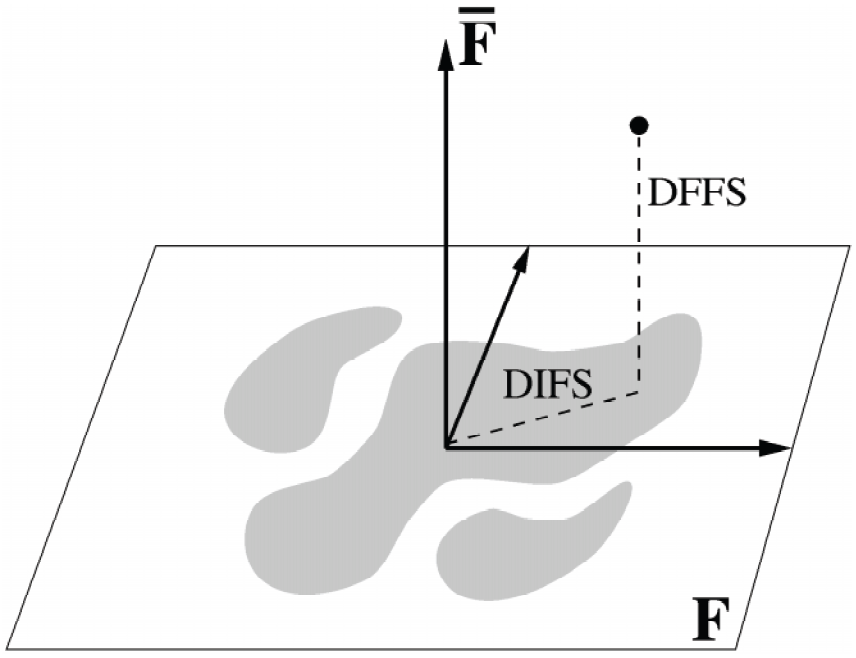
\includegraphics[width=0.5\textwidth]{thesis/1998_JNL_ProbVisLearning_Moghaddam_fig3.png}
								\caption{Graphical illustration of DFFS (distance-from-feature-space) and DIFS (distance-in-feature-space).  The feature space is $\mathbf{F}$ while the subspace orthogonal to the feature space is $\bar{\mathbf{F}}$.  DFFS is the signal residual error and DIFS is the $\mathbf{F}$-space likelihood \cite{1997_JNL_EigenTRK_Moghaddam}.}
					\label{fig:1997_JNL_DIFSDFFS_Moghaddam}
								\end{figure}


%----------------------------------------
\subsection{Brief history}
%----------------------------------------
In this work, we try to address single-target visual-tracking under several of the challenges mentioned above while trying to learn the appearance model of the target.  Seminal work here can be traced back to 1996 when Black and Jepson experimented with tracking using an eigenspace representation of the target appearance model~\cite{1998_JNL_Eigentracking_Black}.  The next notable work is by Moghaddam and Pentland, 1997~\cite{1997_JNL_EigenTRK_Moghaddam} in which they try to address a fundamental limitation of PCA.  In PCA, 2 vectors, $\mathbf{x}_1$ and $\mathbf{x}_2$ can have the same distance to a reduced eigenspace even if they have different distance to the mean of the data.  This is shown for a trivial case in $\mathbb{R}^2$ in Figure~\ref{fig:PRML_PCA_problem} where $\mathbf{e}_1=\mathbf{e}_2=\mathbf{e}$ even though $\mathbf{x}_1$ is closer to the mean $\boldsymbol\mu$ than $\mathbf{x}_2$.  They formulate the problem using DIFS (distance in feature space) and DFFS (distance from feature space) so that both projection error and distance to the mean of the data are used while trying to determine how well the subspace explains a new data-point.  The next breakthrough came with the work of Bishop and Tipping in 1999~\cite{1999_JNL_PPCA_Tipping} where they show that a probabilistic variation of PCA (PPCA) allows PCA to be used as a generative model.  The advantage in tracking is that this methodology allows an assignment of probabilities to new data-points.  This relative weighting can be used to determine best candidates.  All three works were combined into a tracking framework for the first time by Ross et. al. in 2008~\cite{2008_JNL_subspaceTRK_Ross}.  Moreover, they used incremental SVD to make their tracker run in real time.  

Here, we extend this work using RVQ instead of PCA and introducing two new distance based measures for relative weighting of tracking candidates.  The result is a generative framework for RVQ that leads to robust tracking.  Whereas RVQ was first introduced by Juang and Gray in 1982~\cite{1982_CNF_SpeechRVQ_JuangGray}, subsequently greatly extended by the seminal work of Barnes~\cite{1991_CNF_DesignPerformanceRVQ_Frost,1992_JNL_RVQ_Barnes,1992_CNF_ImageCodingRVQ_Kossentini,1993_sigmaTrees_Barnes,1993_JNL_RVQDSC_Barnes,1995_JNL_OptimalityRVQ_Kossentini,1996_CNF_VQclassification_Barnes,1996_JNL_AdvancesRVQ_Barnes,2002_JNL_SigmaTrees_Barnes,2004_CNF_DSSAdataMining_Barnes,2007_JNL_Katrina_Barnes,2007_JNL_IDDM_Barnes} and widely known in the signal processing and information theory communities, relatively little attention has been given to this work in the computer vision and machine learning fields where a much simpler version, K-means, has been widely used.  Our goal is to remedy this situation and introduce RVQ in the context of an important and challenging problem, visual target tracking.

								\begin{figure}[t]
								\centering
	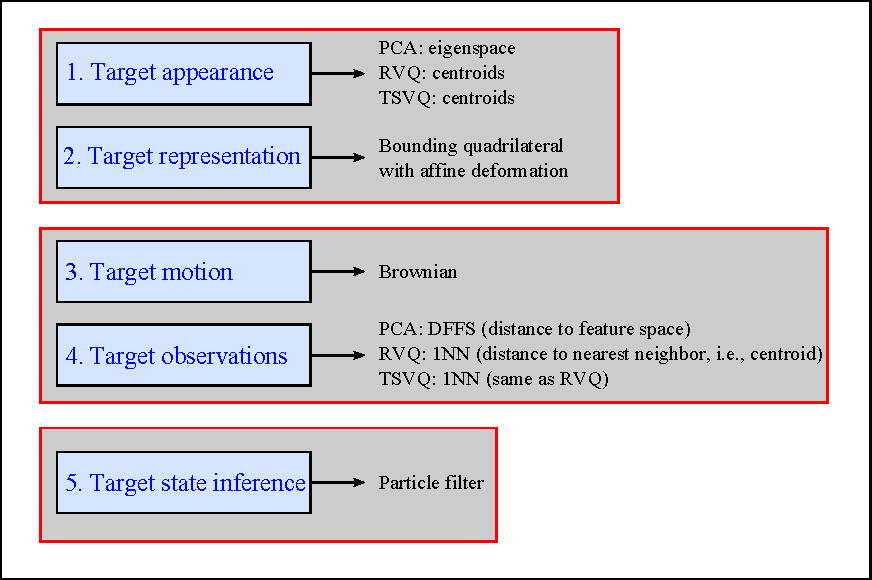
\includegraphics[width=1.0\textwidth]{thesis/PhD_experimentalOverview.pdf}
								\caption{Overview.}
								\label{fig:overview}
								\end{figure}

								\begin{figure}[t]
								\centering
								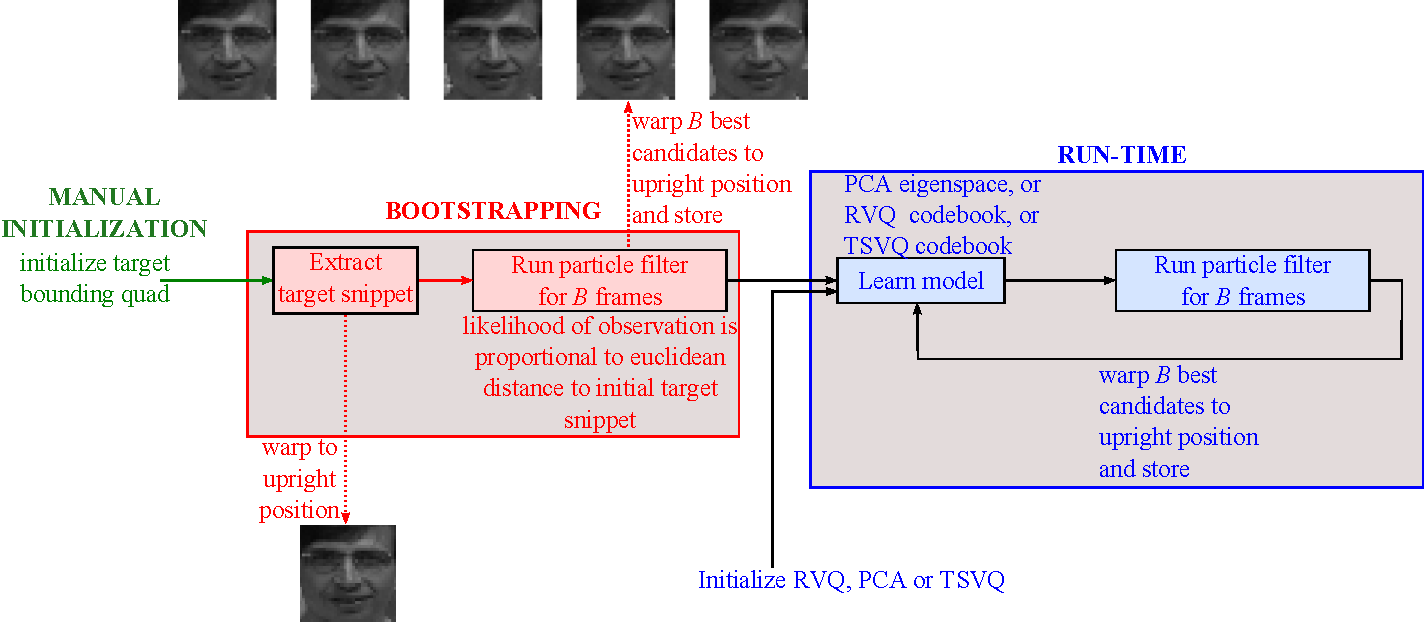
\includegraphics[width=1\textwidth]{thesis/PhD_experimentalTemporalOverview.pdf}
								\caption{Temporal overview.}
								\label{fig:temporal_overview}
								\end{figure}
%----------------------------------------------------
\subsection{Overview of approach used}
%----------------------------------------------------
Our tracking framework is based on five components as shown in Figure~\ref{fig:overview} .  Each of these components is described in detail in later sections.  Here, we present an overview of each:

\begin{enumerate}
\item \underline{ Target appearance}.  Target appearance is modeled using a learned eigenspace, a trained $\sigma$-tree codebook or a binary balanced-tree TSVQ codebook for PCA, RVQ and TSVQ respectively.  Refer to Chapter~\ref{chap_RVQ} for a description of RVQ  $\sigma$-trees.

\item \underline{Target representation}.  Several target representation methods are described in Chapter~\ref{chap_Introduction}.  We use the bounding quadrilateral method.  This quad encloses the pixels of a target of interest.  It is also allowed to warp affinely from frame to frame to minimize inclusion of background pixels as the target changes shape, size and orientation.

\item \underline{Target motion}.  In order to keep our work general, we do not assume any deterministic target motion model.  The target is expected to move according to a Wiener process, i.e., brownian motion.  This allows for robust tracking under arbitrary target and camera motion.

\item \underline{Target observations}.  For PCA, the likelihood of a target observation is assumed proportional to the DFFS (distance to feature space).  DFFS is explained in Chapter~\ref{chap_TRK}.  For RVQ, the likelihood of a target observation is assumed to be proportional to the Euclidean distance to the closest equivalent code-vector.  Equivalent code-vectors are explained in Chapter~\ref{chap_RVQ}.  For TSVQ, the likelihood of a target observation is assumed to be proportional to the Euclidean distance to the closest terminal code-vector.

\item \underline{Target state inference}.  In tracking, the correspondence of observations in the current frame to existing targets in the previous frame is generally an ill-posed problem~\cite{2005_CNF_TRK_Yang}.  We use the particle filter to deal with this problem by propagating multiple hypotheses from frame to frame~\cite{1998_JNL_Condensation_IsardBlake}.

\end{enumerate}

%----------------------------------------------
\subsection{Overview of temporal process}
%----------------------------------------------
In the previous section, we described the five major components of our visual tracking framework.  In this section, we describe the temporal relationship between these components.  Refer to Figure~\ref{fig:temporal_overview} for a graphical overview.  A brief description of this temporal process is given below while detailed explanation is given in later sections in this chapter.

\begin{enumerate}
\item \underline{Manual initialization}.  The target is identified in the first frame by manually drawing a bounding box around it.

%The box is allowed to be affinely deformed as discussed later in this chapter.  Template matching then allows a certain number of frames to be designated as initial training frames.  Currently this value is set to $N_B=5$. 

\item \underline{Bootstrapping}.  A particle filter is run for $B$ frames.  The likelihood of observations is assumed to be proportional to the Euclidean distance from the manually segmented target in the first frame.  The $B$ MAP estimates, i.e. $B$ snippets, one from each of the $B$ frames is stored.

  \item \underline{Run-time}.  During this step, the learning process and the particle run alternately.  For PCA, the learning process includes updating its eigenbasis with the MAP estimates of the particle filter.  For RVQ and TSVQ, the learning process includes updating their codebooks. 
\end{enumerate}


%This model ties in multiple possible spatial observations in a temporal framework to enable sequential inference through the tracking process.
%Every frame after the one-time initialization is tested against the iPCA, bPCA, RVQ and TSVQ models and results are compared.  The Condensation algorithm is used for temporal and spatial integration of observation and state information.  Spatial processing includes generating several candidate window chips (snippets) and picking the one that gives least mean squared reconstruction error.  Temporal processing includes carrying over the posterior density from a frame as the prior density for the next frame.  The snippet that gives the least squared error is retained and added to the pool of training images in FIFO (first-in first-out) fashion, i.e. a moving window of $N_w$ training images is maintained.

The integration of the above-mentioned 5 components in the temporal process just explained enables us to handle the following tracking challenges:

\begin{itemize}
\item \underline{Target appearance related}: Target pose changes, lighting changes, structured noise and temporary occlusions.
\item  \underline{Target representation related}: Target scale and orientation changes.
\item  \underline{Target motion related}: Arbitrary camera and target motion.
\end{itemize}

We now discuss each component in our tracking framework (Figure~\ref{fig:overview}).  

%============================
\section{Model 1: Appearance model}
\label{Sec:RVQ_trk_appearance_model}
%============================
\begin{figure}[t]
\subfigure[Uniform random variable $U\sim$ \texttt{[}0, 1\texttt{]} in $\mathbb{R}^{1089}$, 100 realizations.]{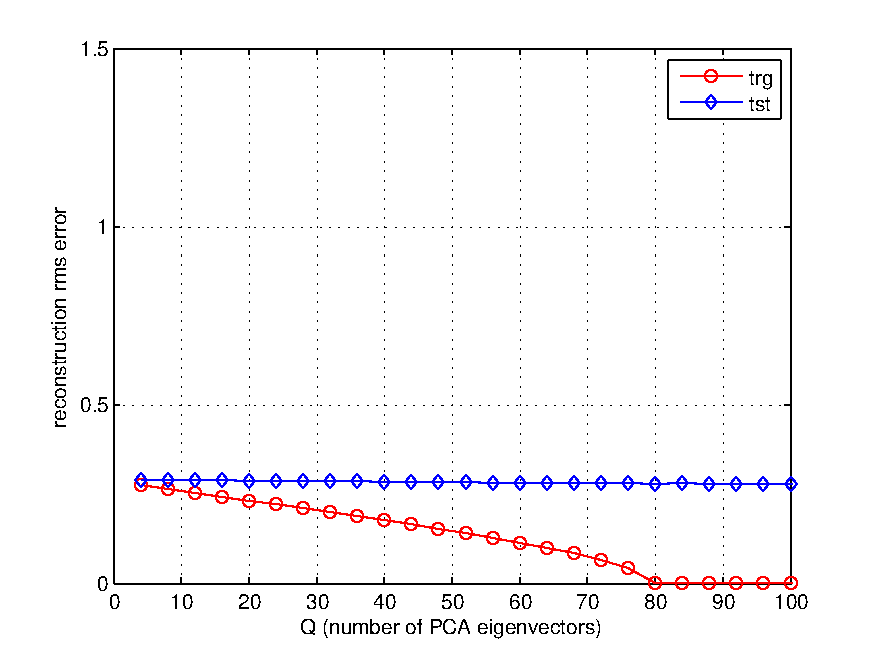
\includegraphics[width=0.45\textwidth]{thesis/PCA_Uniform.pdf}}
\subfigure[Gaussian random variable $\mathcal{N}\sim$(0, 1) in $\mathbb{R}^{1089}$, 100 realizations.]{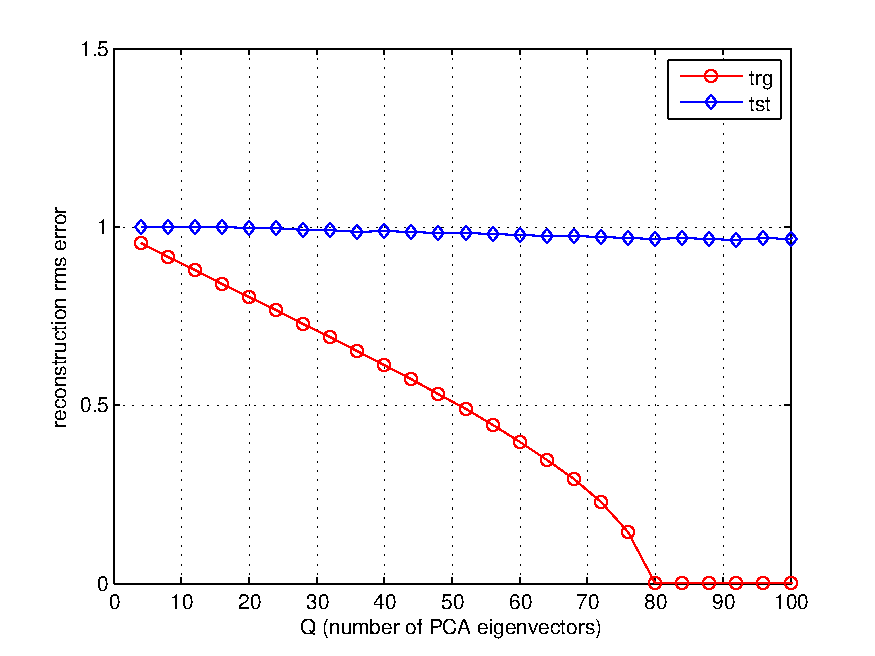
\includegraphics[width=0.45\textwidth]{thesis/PCA_Gaussian.pdf}}
\subfigure[Gauss-Markov random variable $\mathcal{N}\sim$(0, 1) in $\mathbb{R}^{1089}$ with 0.9 correlation, 100 realizations.]{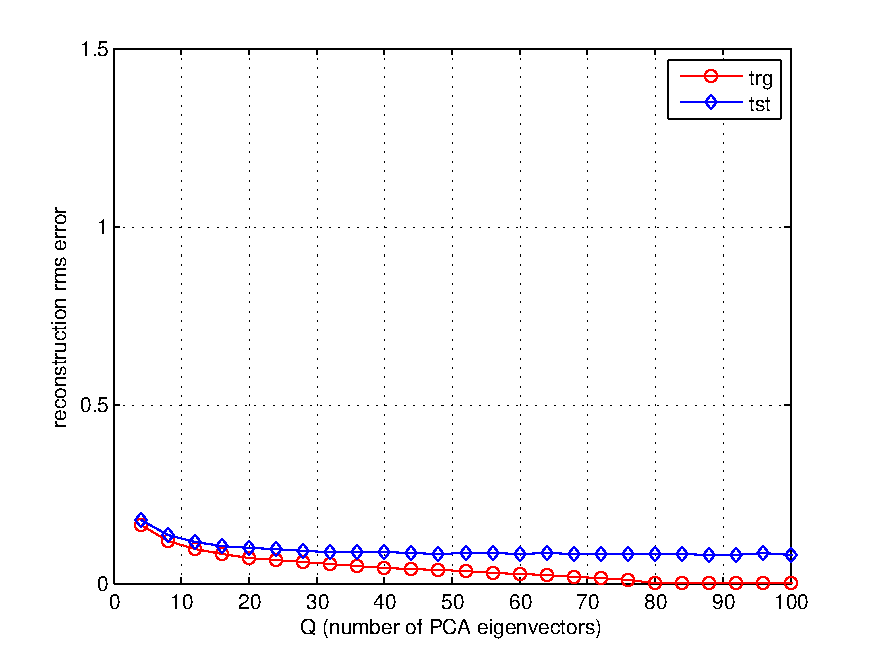
\includegraphics[width=0.45\textwidth]{thesis/PCA_GaussMarkov.pdf}}\hspace{0.55in}
\subfigure[Dudek sequence, 33x33 ($\mathbb{R}^{1089}$) face snippets were extracted from the first 100 images.]{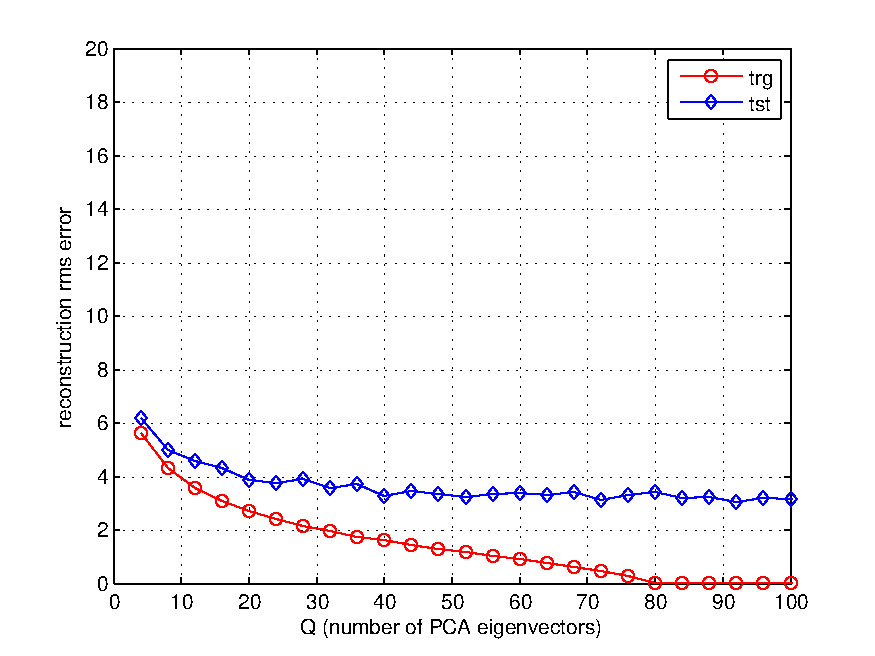
\includegraphics[width=0.45\textwidth]{thesis/PCA_Dudek.pdf}}
\caption{PCA, 100 training examples in $\mathbb{R}^{1089}$ were used for each of these experiments. Results were averaged over 10 cross-validation runs. For each run, 20\% of the data, i.e., 20 examples were randomly picked for testing while the remaining 80 examples were used for training.}
\label{fig:PCA_results}
\end{figure}

\begin{figure}[t]
\subfigure[Uniform random variable $U\sim$ \texttt{[}0, 1\texttt{]} in $\mathbb{R}^{1089}$, 100 realizations.]
{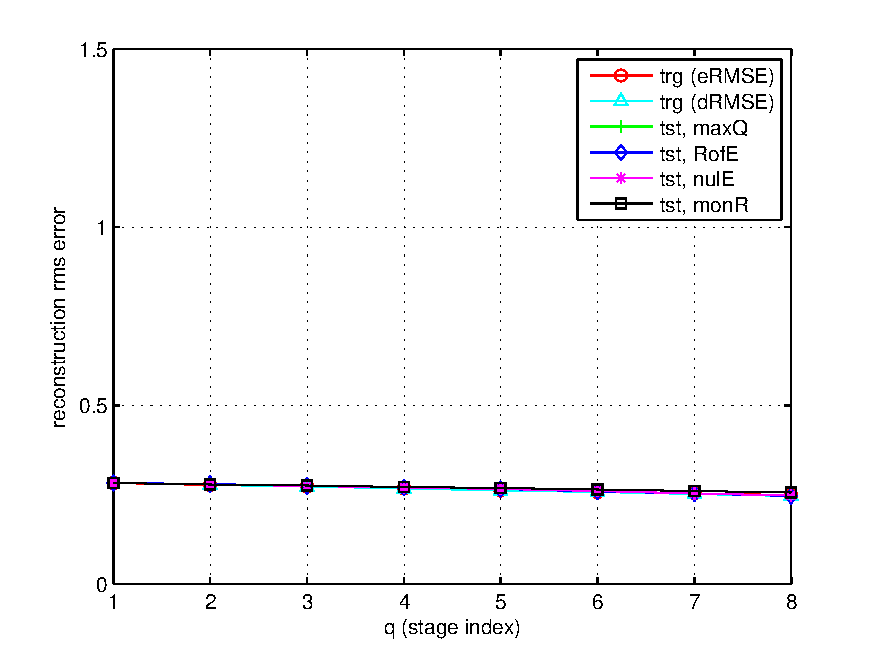
\includegraphics[width=0.45\textwidth]{thesis/RVQ_8x4_Uniform.pdf}}
\subfigure[Gaussian random variable $\mathcal{N}\sim$(0, 1) in $\mathbb{R}^{1089}$, 100 realizations.]
{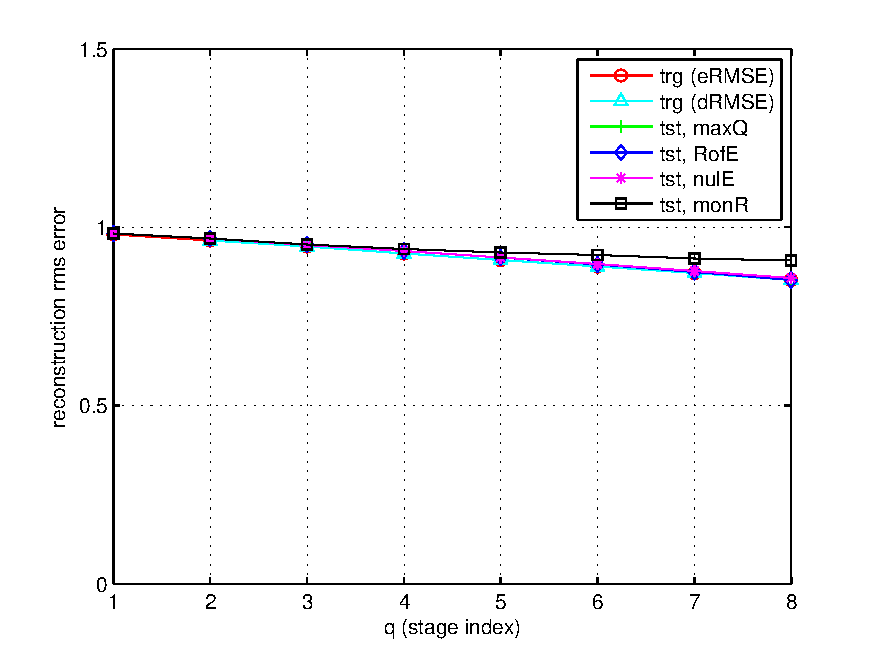
\includegraphics[width=0.45\textwidth]{thesis/RVQ_8x4_Gaussian.pdf}}
\subfigure[Gauss-Markov random variable $\mathcal{N}\sim$(0, 1) in $\mathbb{R}^{1089}$ with 0.9 correlation, 100 realizations.]
{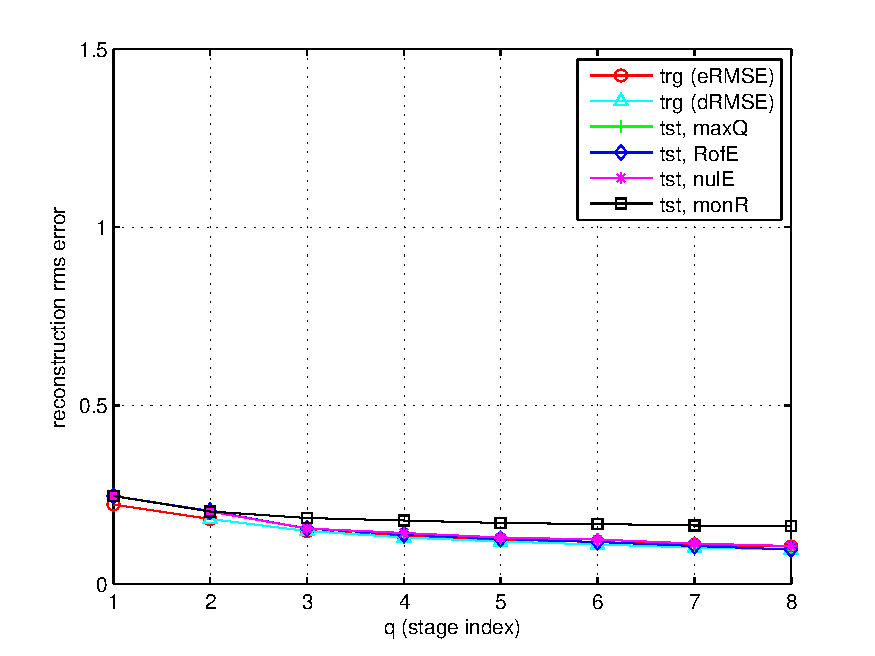
\includegraphics[width=0.45\textwidth]{thesis/RVQ_8x4_GaussMarkov.pdf}}\hspace{0.55in}
\subfigure[Dudek sequence, 33x33 ($\mathbb{R}^{1089}$) face snippets were extracted from the first 100 images.]
{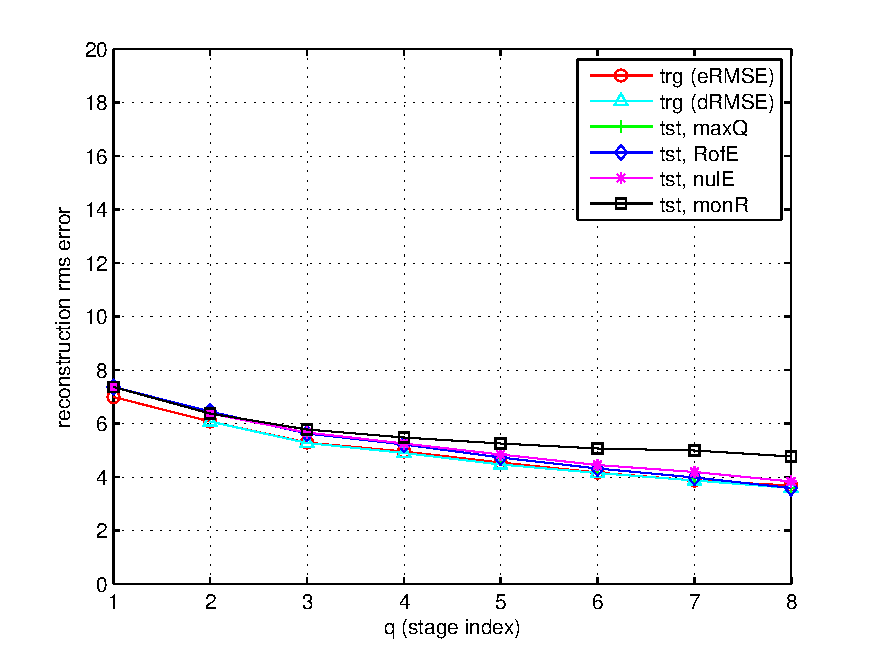
\includegraphics[width=0.45\textwidth]{thesis/RVQ_8x4_Dudek.pdf}}
\caption{RVQp, varying number of stages $P$ with number of code-vectors per stage held constant at $M=4$. 100 training examples in $\mathbb{R}^{1089}$ were used for each of these experiments. A single test example in $\mathbb{R}^{1089}$ was reconstructed.}
\label{fig:RVQ_results_varyingP}
\end{figure}

\begin{figure}[t]
\subfigure[Uniform random variable $U\sim$ \texttt{[}0, 1\texttt{]} in $\mathbb{R}^{1089}$, 100 realizations.]
{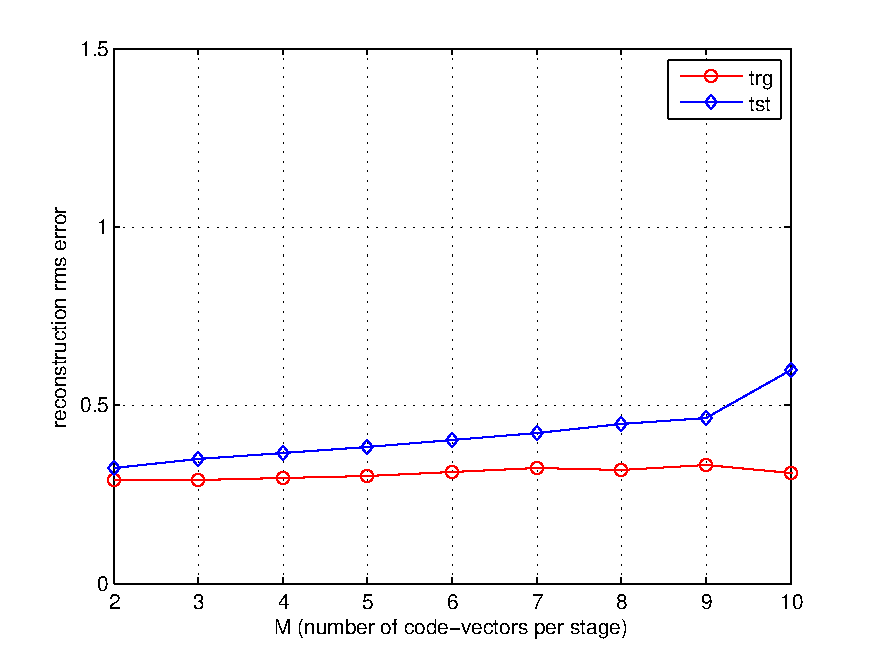
\includegraphics[width=0.45\textwidth]{thesis/RVQ_uniform.pdf}}
\subfigure[Gaussian random variable $\mathcal{N}\sim$(0, 1) in $\mathbb{R}^{1089}$, 100 realizations.]
{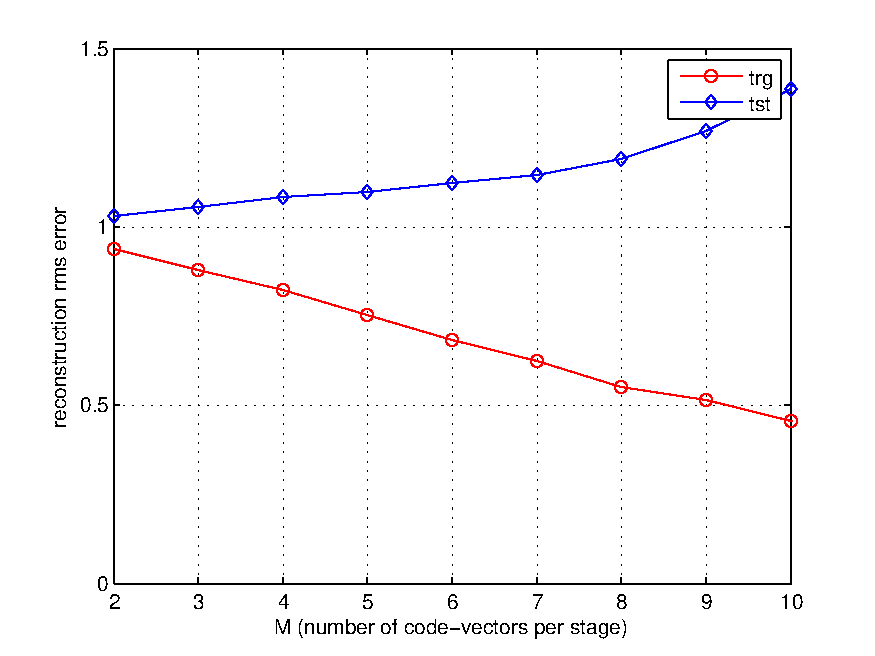
\includegraphics[width=0.45\textwidth]{thesis/RVQ_Gaussian.pdf}}
\subfigure[Gauss-Markov random variable $\mathcal{N}\sim$(0, 1) in $\mathbb{R}^{1089}$ with 0.9 correlation, 100 realizations.]
{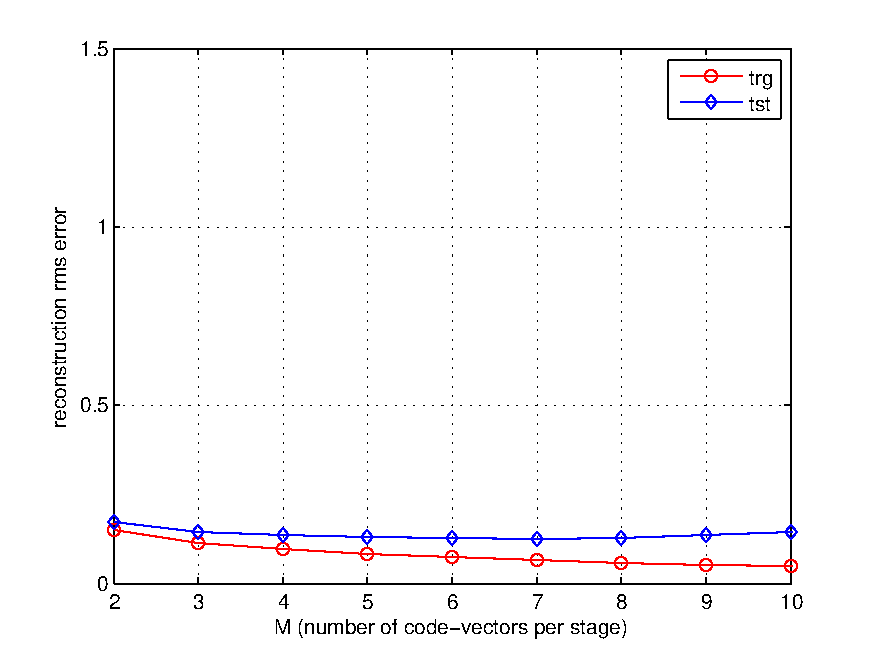
\includegraphics[width=0.45\textwidth]{thesis/RVQ_GaussMarkov.pdf}}\hspace{0.55in}
\subfigure[Dudek sequence, 33x33 ($\mathbb{R}^{1089}$) face snippets were extracted from the first 100 images.]
{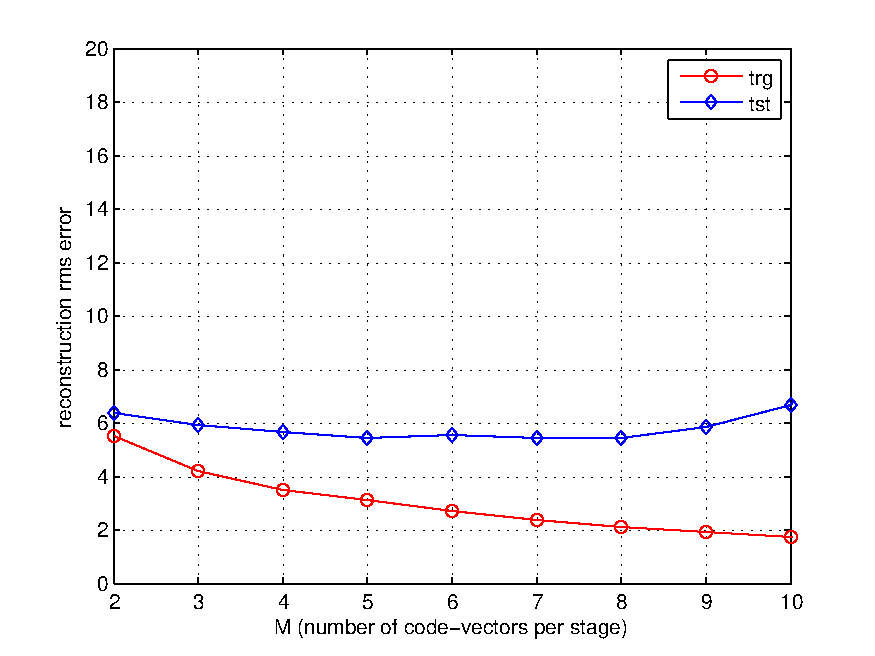
\includegraphics[width=0.45\textwidth]{thesis/RVQ_Dudek.pdf}}
\caption{RVQm, experiments, varying number of code-vectors per stage $M$ with number of stages held constant at $P=8$. 100 training examples in $\mathbb{R}^{1089}$ were used for each of these experiments. Results were averaged over 10 cross-validation runs. For each run, 20\% of the data, i.e., 20 examples were randomly picked for testing while the remaining 80 examples were used for training.}
\label{fig:RVQ_results_varyingM}
\end{figure}

\begin{figure}[t]
\subfigure[Uniform random variable $U\sim$ \texttt{[}0, 1\texttt{]} in $\mathbb{R}^{1089}$, 100 realizations.]{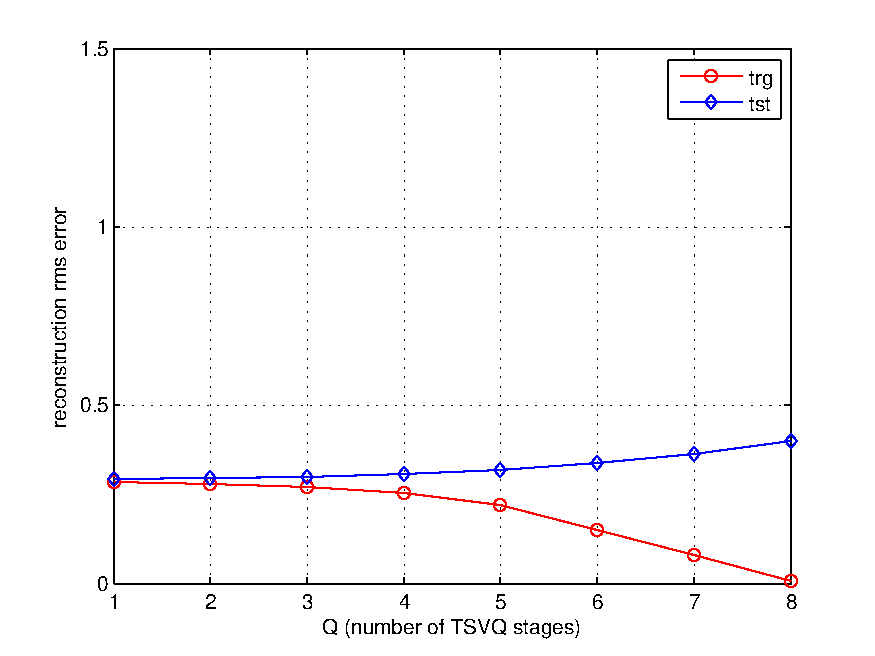
\includegraphics[width=0.45\textwidth]{thesis/TSVQ_Uniform.pdf}}
\subfigure[Gaussian random variable $\mathcal{N}\sim$(0, 1) in $\mathbb{R}^{1089}$, 100 realizations.]{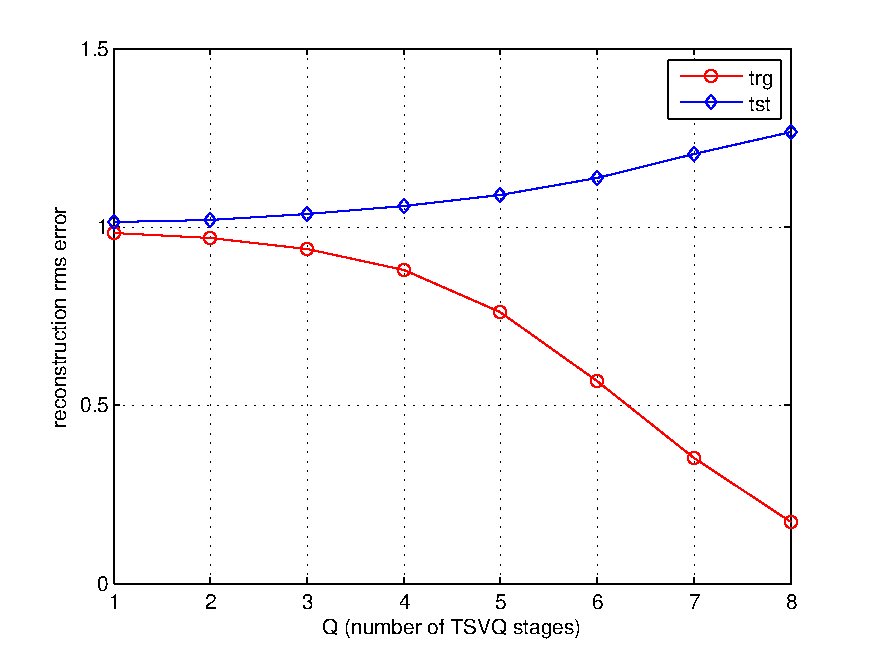
\includegraphics[width=0.45\textwidth]{thesis/TSVQ_Gaussian.pdf}}
\subfigure[Gauss-Markov random variable $\mathcal{N}\sim$(0, 1) in $\mathbb{R}^{1089}$ with 0.9 correlation, 100 realizations.]{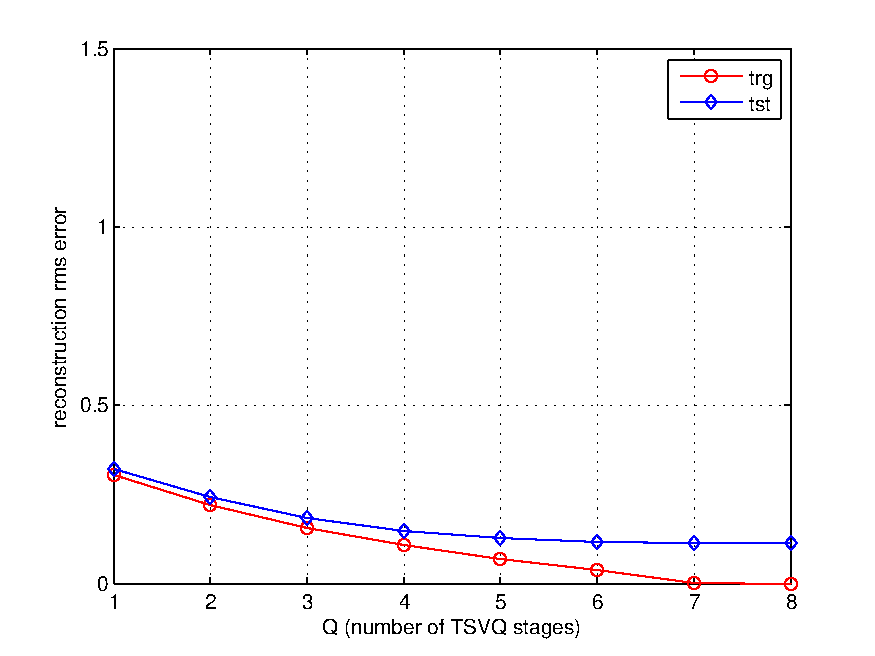
\includegraphics[width=0.45\textwidth]{thesis/TSVQ_GaussMarkov.pdf}}\hspace{0.55in}
\subfigure[Dudek sequence, 33x33 ($\mathbb{R}^{1089}$) face snippets were extracted from the first 100 images.]{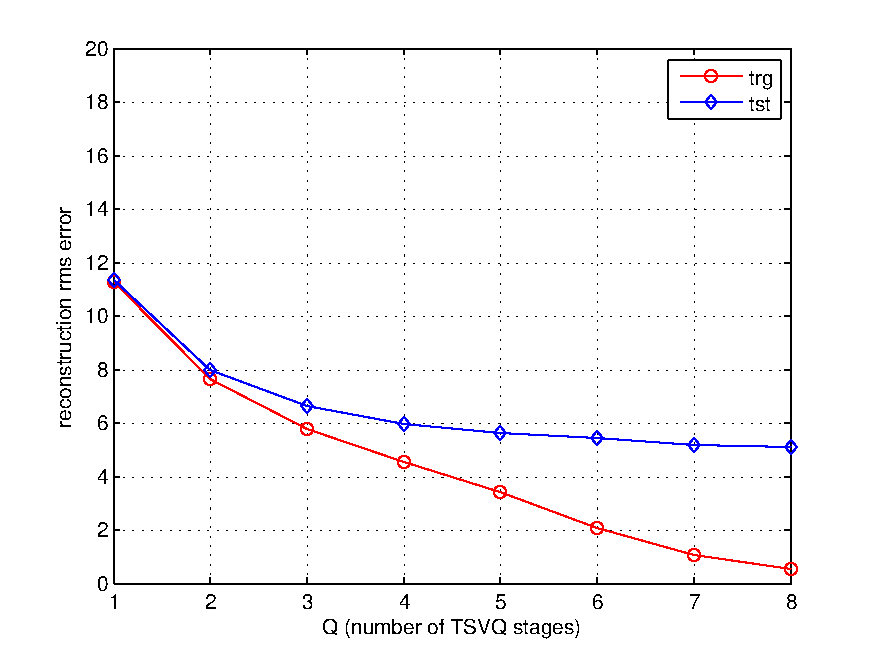
\includegraphics[width=0.45\textwidth]{thesis/TSVQ_Dudek.pdf}}
\caption{TSVQ, 100 training examples in $\mathbb{R}^{1089}$ were used for each of these experiments. Results were averaged over 10 cross-validation runs. For each run, 20\% of the data, i.e., 20 examples were randomly picked for testing while the remaining 80 examples were used for training.}
\label{fig:TSVQ_results}
\end{figure}

Common appearance models include just the raw values of the pixel intensities~\cite{2000_CNF_TRK_Mallet, 1981_JNL_OpticalFlow_HornSchunck}, pixel intensity distributions~\cite{2002_JNL_MeanShiftFeatureSpaceAnalysis_Comaniciu, 1996_JNL_TRK_Zhu, 2002_JNL_TRK_Paragios, 2002_JNL_TRK_Elgammal}, templates\cite{1997_CNF_TRK_Fieguth}, active appearance models\cite{1998_CNF_ActiveModels_Edwards, 1995_JNL_ActiveModels_Cootes}, pixel intensity centroids~\cite{1997_CNF_TRK_Heisele} and subspace based methods~\cite{1997_JNL_EigenTRK_Moghaddam, 1998_JNL_Eigentracking_Black}.  

In order to understand appearance modeling, we conduct the following 4 experiments using PCA, RVQ and TSVQ to measure rms errors for target reconstruction:

\begin{enumerate}
\item PCA: varying number of eigenvectors, $Q$.
\item RVQp: varying number of stages $P$ for RVQ while holding the number of code-vectors per stage constant at $M=4$.
\item RVQm: varying number of code-vectors per stage for RVQ while holding the number of stages constant at $P=8$.
\item TSVQ: varying number of stages, $P$.
\end{enumerate}

It is hoped that investigating reconstruction errors will aid in understanding the behavior of these various algorithms when used to model target appearance in tracking applications.

We use four datasets in $\mathbb{R}^{1089}$: (a) Uniform random variable, (c) Gaussian random variable, (c) Gauss-Markov random variable, and (d) images from the Dudek sequence. The reason for using $\mathbb{R}^{1089}$ is that our targets for all our tracking datasets are warped to a canonical size of 33-pixel height and 33-pixel width (33x33=1089). In all cases, we take 100 examples and split them up using an 80/20 rule, i.e. 80 training examples and 20 test examples. 10 cross-validation runs are used. In each cross-validation run, the training and test examples are picked randomly in the 80/20 ratio.

Results for PCA, RVQp, RVQm and TSVQ are shown in Appendix~\ref{App:plots} as Figures~\ref{fig:PCA_results}, \ref{fig:RVQ_results_varyingP} \ref{fig:RVQ_results_varyingM} and \ref{fig:TSVQ_results} respectively.
We make the following observations from the results:
\begin{enumerate}
\item \textbf{Training error}. Training error is always less than test error, as expected. Also, for each of the algorithms individually, we observe,
\begin{itemize}
\item \underline{PCA}: Monotonic decrease with increasing $Q$. Training error becomes 0 when 80 eigenvectors are used, since there are 80 training examples.
\item \underline{RVQp}: Monotonic decrease with increasing $P$.
\item \underline{RVQm}: Can increase or decrease with increasing $M$, but slight variation.
\item \underline{TSVQ}: Monotonic decrease with increasing $P$.
\end{itemize}
\item \textbf{Test error}.
\begin{itemize}
\item \underline{Statistically independent data}: For the uniform and Gaussian random variables, test error for PCA and RVQp stays almost constant with increasing $Q$ and $P$ respectively. For RVQm and TSVQ, test error increases with increasing $P$. The reason is that PCA and RVQp use successive refinement when increasing $Q$ and $P$ respectively. Test error is therefore not expected to get better since it is not possible to better explain random data with increasing $Q$ and $P$.
On the other hand, RVQm and TSVQ control generalization ability with increasing $Q$, as discussed in an earlier report on VC dimension. Therefore, when the number of code-vectors increases, they tend to explain the training data well and are unable to explain the test data. For both RVQm and TSVQ, notice that when training error falls off sharply, test error increases sharply. Also, when training error drop is gradual, so is test error increase rate. This confirms over-generalization behavior. Also, RVQ increase or decrease rates are more gradual than TSVQ. And finally, the over-generalization for both RVQm and TSVQ is less pronounced with uniform random data than with Gaussian random data since there is more uncertainty in the latter distribution.
\item \underline{Statistically dependent data}: For the Gauss-Markov and Dudek cases, all 4 algorithms display decreasing test error with increasing $Q$ or $P$. The "knee" is visible in all cases.
\end{itemize}
\end{enumerate}
In general, the training and test errors for RVQ are less than TSVQ. This is due to the fact that RVQ has access to all data at every stage while designing codebooks, and can therefore better optimize stage code-vectors. In TSVQ, data is partitioned at every stage and can lead to data starvation.
Training error of PCA is in general better than RVQ. This is expected since PCA can achieve perfect reconstruction when $Q$ comes close to the number of training examples $N$, $N<<D$. Test errors however are comparable.

RVQ has 2 knobs, $P$ and $M$. In varying $P$, it acts like PCA in providing successive approximation. In varying $M$, it acts like TSVQ in changing its VC dimension, and therefore its generalization ability.
Given this flexibility, it is expected that RVQ will perform well in tracking experiments.

%=======================		
\section{Model 2: Observation model}
%=======================
								\begin{figure}
								\centering
								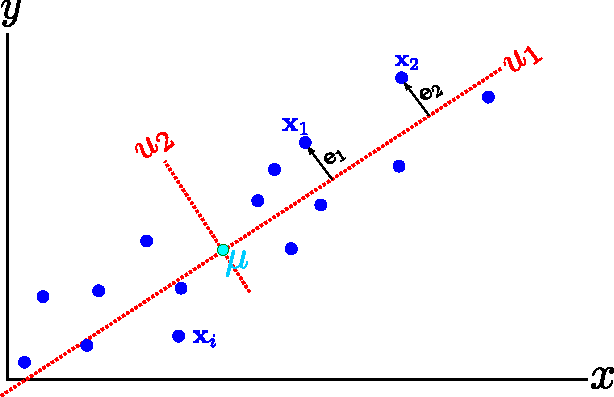
\includegraphics[width=0.45\textwidth]{thesis/PRML_PCA_problem.pdf}
								\caption{In $\mathbb{R}^2$, a reduced eigenspace means that eigenvector $u_2$ is discarded.  Vectors $\mathbf{x}_1$ and $\mathbf{x}_2$ have the same projection error on eigenvector $u_1$ even though $\mathbf{x}_1$ is closer to the mean $\boldsymbol\mu$ of the training data $\mathbf{x}_i$.}
								\label{fig:PRML_PCA_problem}
								\end{figure}
		

In this work, for PCA, it is assumed that an image $\mathbf{X}$ in $R^D$ is probabilistically generated from a subspace $\mathbf{U}$ spanned by earlier observed images.  The covariance matrix $\Sigma$ of the input training images can be written as follows,  

\begin{equation}
\Sigma = \mathbf{U}\mathbf{\Lambda} \mathbf{V}^T
\end{equation}

Here $\mathbf{\Lambda}$ is the matrix of eigenvalues.  The distribution is assumed to be Gaussian centered at $\mathbf{\mu}$.  The probability of an image being generated under this distribution is inversely proportional to its distance from $\mathbf{\mu}$.  This distance can be decomposed into two parts:

\begin{enumerate}
\item DFFS (distance-from-feature-space):  In a partial KL expansion using $Q$ eigenvectors, the space spanned by these $Q$ eigenvectors is given by $\mathbf{F}$ and the signal residual $\epsilon^2$ is given by

\begin{equation}
\epsilon^2 = \Vert \tilde{\mathbf{X}} \Vert^2 - \sum\limits_{i=1}^M \mathbf{u}_i^2 = \sum\limits_{i=M+1}^D \mathbf{u}_i^2
\end{equation}

where $\mathbf{u}_i$ are the eigenvectors of $\Sigma\Sigma^T$ and $\tilde{\mathbf{X}}$ is the mean removed input image.  This signal residual is referred to as DFFS.
\item DIFS (distance-in-feature-space):  This is the component of $\mathbf{X}$ which lies in the feature space $\mathbf{F}$.  
\end{enumerate}

DIFS and DFFS are illustrated graphically in Figure~\ref{fig:1997_JNL_DIFSDFFS_Moghaddam}.  

%This leads the likelihood function to be a function of two distributions,
%
%\begin{equation}
%p(\mathbf{I}|\mathbf{X}) =  \mathcal{N}()
%\end{equation}
%
%\begin{equation}
%p(I_t|X_t) = \mathcal{N}
%\end{equation}

For RVQ, the appearance model is exactly the same as that used in Chapter~\ref{chap_RVQ_CV_recog}.  The only difference is that the codebooks are now dynamic and updated every $N_B=5$ frames. 


The Tree Structured Vector Quantizer (TSVQ) has received a lot of attention in the literature~\cite{1991_BOOK_VQ_GershoGray}.  The reason is that the codebook produced by a TSVQ approximates the codebook produced by an Exhaustive Search Vector (ESVQ) but the run-time computational cost is logarithmic in the number of code-vectors.  The storage requirements however are greater.  A comparison of ESVQ, TSVQ and RVQ can be seen in Table~\ref{tab:comparison_ESVQ_TSVQ_RVQ}.

In TSVQ design, the first step is to compute the mean of the data.  All the data is mapped to this mean.  The mean is then split off into $M_{TSVQ}$ centroids (code-vectors).  For a binary TSVQ, $M=2$.  The data is mapped to these centroids using the Nearest Neighbor rule.  Each of these $M_{TSVQ}$ parent centroids is then again split into $M_{TSVQ}$ child centroids.  Splitting can be achieved by multiple iterations of the K-means algorithm to get centroids that give low mean squared error.  At every stage of the tree, data belonging to a parent code-vector is mapped to the child code-vectors after the splitting occurs.  Notice that the important code-vectors are the last stage children code-vectors, i.e. the terminal leaves of the tree.  However, during run-time, the parent code-vectors, i.e., the non-terminal nodes of the tree have to be stored in order to be able to traverse the tree to get to the terminal code-vectors.  The process of mapping data at run-time to the terminal code-vectors is quite straightforward.  The data is first mapped to the mean, which is a trivial step, since all data starts at the top of the tree, i.e., the mean.  Each data-point is then mapped to one of the two children nodes at the first stage using the Nearest Neighbor method.  This process continues till a terminal code-vector is reached which is then used as an approximation to the input data-point.

In this work, we use a binary and balanced TSVQ.  In the binary case, the storage requirements are double the storage requirements for an equivalent ESVQ.  However, the run-time savings decrease logarithmically.  For instance, a codebook size of $K=256$ requires 256 matches for ESVQ but only 8 matches for a binary TSVQ.  

During tracking, a TSVQ codebook is designed every $N_B=5$ frames using $N_w$ images in the training buffer.  The particle filter candidate target regions in the current frame are tested against this code-book, i.e., for each candidate region, the terminal code-vector  to the mean squared error between that region and the terminal code-vector in the tree that 

The candidate that gives least mean squared error is chosen as the most likely  to find the terminal code-vector in the TSVQ tree that minimizes mean-squared error.  

An observation model $p(z_t|x_t)$ relates the state $x_t$ at time $t$ to the observation $z_t$ at time $t$.  Unfortunately, it is not possible to estimate it from the data and so reasonable assumptions must be made.  The observations are assumed to be independent of each other as well as of the dynamical process \cite{1998_JNL_Condensation_IsardBlake}. 

In this work, for PCA, the observation model assumes that the candidate window chips (snippets) in the image that can contain the target were generated from a subspace of the target $\mathbf{U}$ centered at $\mathbf{\mu}$.  The distance metric used to score each candidate window is explained in Section~\ref{Sec:Chap5_PCA}.  For RVQ and TSVQ, the observation model assumes that the candidate snippets were generated from the RVQ and TSVQ codebooks respectively.  The distance metric used to score snippets is based on the mean squared reconstruction error.  For RVQ, an additional constraint is monotonic SNR increase in the DSSA (direct sum successive approximation) reconstruction.  In other words, not all RVQ stages have to be used to reconstruct the target.  The reconstruction must stop if the stage code-vector at the next additive stage does not result in SNR increase.


It has been shown by Roweis and Ghahramani~\cite{1999_JNL_Gaussian_roweis} that under the assumption of gaussian noise, factor analysis (FA), principal component analysis (PCA), mixtures of gaussian (MoG) clusters, vector quantization (VQ), independent components analysis (ICA), Kalman filters and hidden Markov models (HMMs) are instances of a single basic generative model, the linear gaussian model.  The linear gaussian model can be written as,

\begin{equation}
\begin{array}{llllllllllllll}
\mathbf{x}_{t+1} &=  \mathbf{A}\mathbf{x}_{t} +  \mathbf{w}_t   & & & \mathbf{w}_t \sim \mathcal{N}(0, \mathbf{Q})\\
\mathbf{y}_t 		 &=  \mathbf{C}\mathbf{x}_{t} +  \mathbf{v}_t    & & & \mathbf{v}_t \sim \mathcal{N}(0, \mathbf{R})
\end{array}
\label{LGM}
\end{equation}

where $\mathbf{A}$ is the state transition matrix, $\mathbf{C}$ is the observation matrix, and $\mathbf{w}_t$ and $\mathbf{v}_t$ are zero-mean gaussian random variables.  Under conditions where each data point $\mathbf{x}$ was generated independently and identically without any temporal ordering, i.e., $\mathbf{A}=\mathbf{0}$, we can write,

\begin{equation}
\begin{array}{llllllllllllll}
\mathbf{x} &= \mathbf{w} 											& & & \mathbf{w} &\sim \mathcal{N}(0, \mathbf{Q})\\
\mathbf{y} &=  \mathbf{C}\mathbf{x} +  \mathbf{v} 		& & & \mathbf{v} & \sim \mathcal{N}(0, \mathbf{R})
\end{array}
\label{LGM1}
\end{equation}



\begin{table}[t]
\centering
\begin{tabular}{| c | c | c | c | c |}\hline
 				 	&\textbf{A}	 	&	\textbf{C}  									& \textbf{Q} 	&  \textbf{R}                                                                		\\\hline
\textbf{PCA} 	&\textbf{0}		&	principal eigenvectors of $\boldsymbol\Sigma$	& \textbf{I}  	&  $\lim\limits_{\sigma^2 \rightarrow 0} \sigma^2\mathbf{I}$ 	\\\hline
\textbf{PPCA} &\textbf{0}		& 	scaled principal eigenvectors of $\boldsymbol\Sigma$	& \textbf{I}	&										      $\sigma^2 \mathbf{I}$	 \\\hline
\textbf{FA}   	&\textbf{0}		&													& \textbf{I} 	&  diagonal matrix 																\\\hline
\textbf{VQ}	 	&\textbf{0} 	&	cluster means								& \textbf{I}	& 	-																					\\\hline
\end{tabular}
\caption{Unifying PCA, PPCA, FA, and VQ using linear gaussian models~\cite{1999_JNL_Gaussian_roweis, 1999_JNL_PPCA_Tipping}.}
\label{table:LGM_unifying}
\end{table}

Moreover, for non-linear mappings, such as in MoG and VQ, a function $\mathbf{WTA[.]}$, \emph{winner-take-all} is introduced which returns a vector with unity in one position and all remaining zeros,

\begin{equation}
\begin{array}{llllllllllllll}
\mathbf{x} &= \mathbf{WTA}(\mathbf{w}) 						& & & \mathbf{w} &\sim \mathcal{N}(\mathbf{\boldsymbol\mu}, \mathbf{Q})\\
\mathbf{y} &=  \mathbf{C}\mathbf{x} +  \mathbf{v} 		& & & \mathbf{v} & \sim \mathcal{N}(0, \mathbf{R})
\end{array}
\label{LGM2}
\end{equation}

The values for \textbf{A}, \textbf{C}, \textbf{Q} and \textbf{R} under this elegant, unifying generative framework for various algorithms, including PCA and VQ, are given in Table~\ref{table:LGM_unifying}.  Besides being inherently satisfying, this framework allows the computation of data likelihoods in the case of PCA and VQ since they both do not define a proper density in the observation space~\cite{1999_JNL_Gaussian_roweis}.  We start with likelihoods under PCA, PPCA and VQ.  Our contribution is extending this work to compute likelihoods under RVQ.


In a gaussian distribution, the probability of a data point $\mathbf{x}$ in $\mathbb{R}^D$ depends on the Mahalanobis distance $d$.  The output of PCA, zero-centered $\mathbf{\tilde{y}}$ is decorrelated with variances along each dimension equal to the eigenvalues $\lambda_i$ of the covariance matrix $\boldsymbol\Sigma$,


\begin{equation}
\begin{array}{lllllll}
d &= (\mathbf{x}-\boldsymbol\mu)^T\boldsymbol\Sigma^{-1}(\mathbf{x}-\boldsymbol\mu)\\
&=\mathbf{\tilde{x}}^T\boldsymbol\Sigma^{-1}\mathbf{\tilde{x}}\\
&=\mathbf{\tilde{x}}^T(\mathbf{U}\boldsymbol\Lambda\mathbf{U}^T)^{-1}\mathbf{\tilde{x}}\\
&=\mathbf{\tilde{x}}^T(\mathbf{U}\boldsymbol\Lambda^{-1}\mathbf{U}^{-1})\mathbf{\tilde{x}}\\
&=(\mathbf{U}^T\mathbf{\tilde{x}})^T\boldsymbol\Lambda^{-1}(\mathbf{U}^T\mathbf{\tilde{x}})	\\
&=\mathbf{\tilde{y}}^T\boldsymbol\Lambda^{-1}\mathbf{\tilde{y}}\\
&=\sum\limits_{d=1}^D \frac{\tilde{y}_i}{\lambda_i}\\
&=\sum\limits_{d=1}^Q \frac{\tilde{y}_i^2}{\lambda_i} + {\color{red}\sum\limits_{d=Q+1}^D} \frac{{\color{red}\tilde{y}_i^2}}{\lambda_i}, \ \ \  & \bigg(\textrm{DFFS = recon. error}={\color{red}\sum\limits_{i=1}^D e_i^2} = \sum\limits_{i=1}^D \tilde{x}_i^2 - \sum\limits_{i=1}^Q \tilde{y}_i^2= {\color{red}\sum\limits_{d=Q+1}^D} {\color{red}\tilde{y}_i^2}\bigg)\\
&=\sum\limits_{d=1}^Q \frac{\tilde{y}_i^2}{\lambda_i} + \frac{1}{\rho} {\color{red}\sum\limits_{i=1}^D e_i^2} \ \ \ & \bigg(\rho^* = \frac{1}{D-q}\sum\limits_{i=q+1}^D \lambda_i\bigg)\\
\end{array}
\label{Eqn:MoghaddamLikelihood}
\end{equation}

This formulation, first presented in~\cite{1997_JNL_EigenTRK_Moghaddam} shows that the first term in the sum is the DIFS term in Figure~\ref{fig:1997_JNL_DIFSDFFS_Moghaddam} while the second term corresponds to DFFS.  With this formulation, PCA can be used in a probabilistic framework since the error of a test vector $\mathbf{x}$ now also depends on its distance from the mean of the data.


For PCA, using Equation~\ref{LGM1} and Table~\ref{table:LGM_unifying}, we have the likelihood of observing $\mathbf{y}$ given by,

\begin{equation}
p(\mathbf{y}) \sim \mathcal{N}(\boldsymbol\mu, \mathbf{C}\mathbf{C}^T + \sigma^2 \mathbf{I})
\end{equation}

Bishop and Tipping~\cite{1999_JNL_PPCA_Tipping} show that this can be done in closed form using PPCA with the following solution,

\begin{equation}
\begin{array}{lllll}
\mathbf{\boldsymbol\mu}_{\textrm{ML}} &=\frac{1}{N}\sum\limits_{i=1}^N \mathbf{x}_i\\
\sigma^2_{\textrm{ML}} &= \frac{1}{D-q}\sum\limits_{i=q+1}^D \lambda_i\\
\mathbf{C}_{\textrm{ML}} &= \mathbf{U}_q(\mathbf{\Lambda}_q - \sigma^2\mathbf{I})^{1/2} \\
\end{array}
\label{Eqn:PPCA}
\end{equation}

where, $\boldsymbol\Sigma = \mathbf{U}\mathbf{\Lambda}\mathbf{V}^T$, $\mathbf{U}_q$ are the first $q$ eigenvectors in $\mathbf{U}$, $\mathbf{\Lambda}_q$ contains the corresponding eigenvalues, $\lambda_1, \lambda_2, \ldots \lambda_q$, $D$ is the dimensionality of the data and $N$ is the number of data points.  Note that in the above equation, we have omitted multiplication with an arbitrary rotation matrix since it can be taken to be $\mathbf{I}$ without loss of generality.  

In Equation~\ref{Eqn:PPCA}, $\sigma^2_{\textrm{ML}}$ is the average variance in the discarded dimensions and $\mathbf{C}_{\textrm{ML}}$ maps $\mathbf{x}$ onto its principal components to give output $\mathbf{y}$.

As mentioned earlier, VQ does not define a proper density in the observation space.  Moreover, in the linear gaussian model, Table~\ref{table:LGM_unifying} shows that in VQ, similar to PCA, the observation noise vanishes, $\lim\limits_{\sigma^2 \rightarrow 0} \sigma^2\mathbf{I}$.  The posterior therefore collapses to a single point, and all its mass is centered on the nearest centroid.  In this case, the likelihood of a data point $\mathbf{x}_i$ is proportional to its squared distance from the nearest centroid.

In this work, we introduce a new distance measure $d_r$ for RVQ.  Its role is similar to the role played by the Mahalanobis distance in probabilistic PCA.  Essentially, it is used to assign a probability measure to a new data point and demonstrates how well this data point is explained by the RVQ codebook $\Phi$.  The RVQ codebook $\Phi$ is generated using training data and 3 parameters, target decoding SNR, $S$, maximum number of stages, $Q_{\textrm{max}}$ and number of codevectors per stages, $M$.  $d_r$ is given by,




\begin{equation}
d_r = \dr
\end{equation}

Here, $\boldsymbol\mu_k$ is closest centroid to $\mathbf{x}_i$, $Q_i$ is the number of stages required to decode $\mathbf{x}_i$, and $\lambda$ is a regularization parameter.  With this distance measure, the likelihood of a data point being generated by an RVQ codebook $\Phi$ is given by,

\begin{equation}
p(\mathbf{x}_i|\Phi) = \frac{e^{-\big(\dr\big)}} {\sum\limits_{i=1}^N e^{-\big(\dr\big)}}
\end{equation}

\begin{enumerate}
\item \underline{maxQ}: In this method, RVQ decoding is carried out so that maximum stages $Q$ are used.
\item \underline{RofE}: In this method, realm of experience coding is used.  A test vector is decoded such that the decode path traversed belongs to the set of training decode paths.
\item \underline{nulE}: In this method, null encoding is used.  Reconstruction rms error is checked at every stage.  If at any stage, rms error is not reduced, that stage is skipped until maximum stages are attained.
\item \underline{monR}: In this method, monotonic rms error is a condition.  If this condition is not met, decoding stops.
\end{enumerate}

%=======================		
\section{Model 3: Representation model}
\label{Sec:Representation_model}
%=======================
%\begin{itemize}
%\item \underline{Temporary occlusions}.  The occlusions are temporary, on the order of about 10 frames.
%\end{itemize}
%\begin{itemize}
%\item \underline{Perspective changes handled effectively with affine deformation}.  An affine transform in a tracking scenario can deal effectively with a large variety of target deformations, including some perspective effects.  We therefore choose the affine transform in favor of the less restrictive projective transform which can handle severe perspective effects.  A comparison of some 2D geometric transformations is given in Table~\ref{table:2Dtransformations}.
%\end{itemize}		
In this section, we discuss the representation model.  We refer back to Figure~\ref{fig:TRK_objectRepresentations} in the introductory chapter that shows different target representations.  




								\begin{figure}[t]
								\centering
								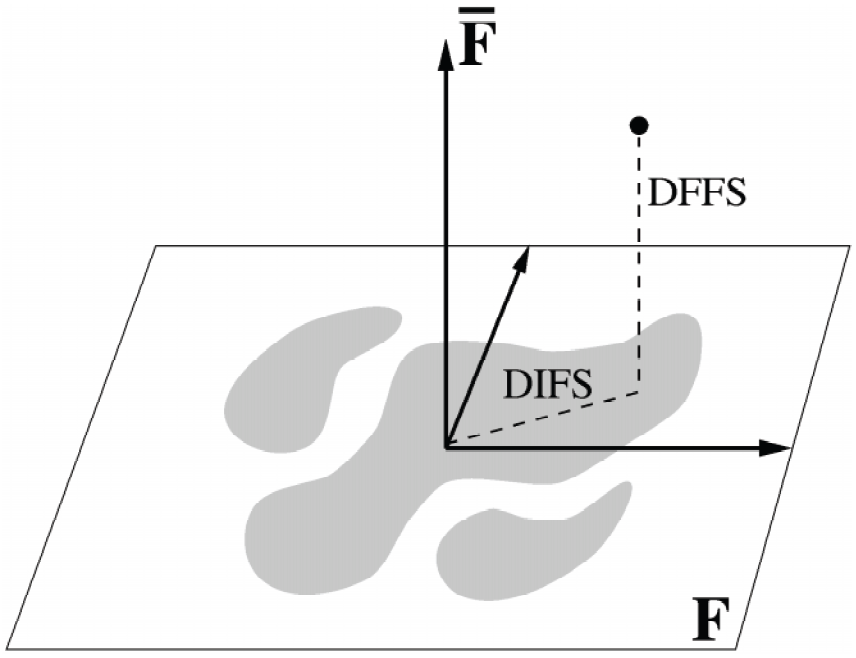
\includegraphics[width=0.5\textwidth]{thesis/1998_JNL_ProbVisLearning_Moghaddam_fig3.png}
								\caption{Graphical illustration of DFFS (distance-from-feature-space) and DIFS (distance-in-feature-space).  The feature space is $\mathbf{F}$ while the subspace orthogonal to the feature space is $\bar{\mathbf{F}}$.  DFFS is the signal residual error and DIFS is the $\mathbf{F}$-space likelihood \cite{1997_JNL_EigenTRK_Moghaddam}.}
								\label{fig:1997_JNL_DIFSDFFS_Moghaddam}
								\end{figure}



In many situations, it is necessary to track a visual target that is undergoing deformations.  Several targets of interest fall in this category, particularly non-rigid targets such as humans.  Even rigid objects can undergo severe deformation in a matter of seconds as shown in Figure~\ref{Fig:PETS2001_deformation}.  


								\begin{figure}
								\centering
								\subfigure[Frame 770.]{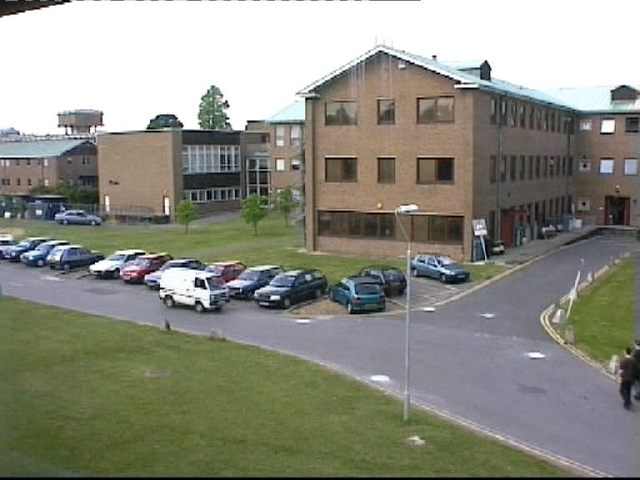
\includegraphics[width=0.45\textwidth]{figs/PETS2001_00770.jpg}}
								\subfigure[Frame 1770.]{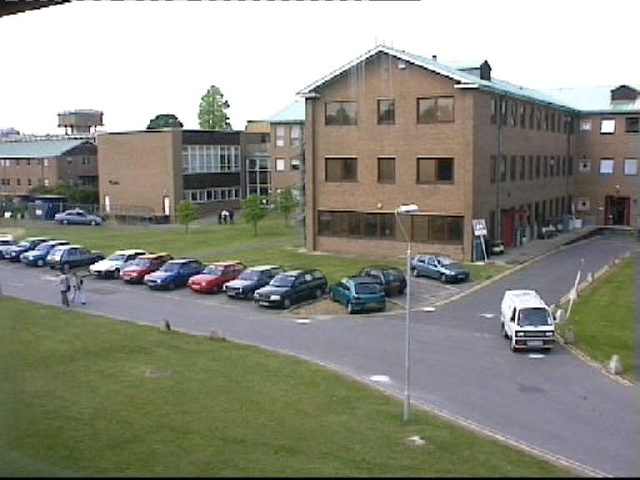
\includegraphics[width=0.45\textwidth]{figs/PETS2001_01770.jpg}}
								\caption{Over time, even rigid objects can undergo severe deformations such as the car in these images from the PETS2001 dataset.}
								\label{Fig:PETS2001_deformation}
								\end{figure}

In such cases, using a rigid rectangular bounding box to represent the target will inevitably lead to inclusion of background pixels in the matching process.  This can easily lead to tracker drift, particularly if the tracker is also trying to learn the appearance model of the target.

We now show how to use affine warping of the rectangular bounding box so that it more closely captures the outline of the target of interest.  This minimizes inclusion of background pixels in the matching process and leads to more robust tracking.


Table \ref{table:2Dtransformations} shows different kinds of 2D linear transformations.  Every transformation generalizes the transformation below it in the table.  In this report, we are interested in the 2D affine transform since it is flexible enough to account for most distortions in real images.

								\begin{table}[t]
								\centering
								\begin{tabular}{| l | c | c | p{2.5in} |}
								\hline
								Transformation & DoF & Matrix & Distortion\\ \hline 
								& & & \\ Projective & 8 & $\ProjMatrix$ & any arbitrary quadrilateral as long as no three points are collinear\\  & & & \\ \hline
								& & & \\ Affine & 6 & $\AffMatrix$ & rotation and non-isotropic scaling\\  & & & \\ \hline
								& & & \\ Similarity & 5 & $\SimMatrix$ & scaling and rigid motion\\  & & & \\ \hline
								& & & \\ Euclidean & 4 & $\EucMatrix$ & rigid motion (rotation, translation) \\  & & & \\ \hline
								\end{tabular}\
								\caption{2D transformations}
								\label{table:2Dtransformations}
								\end{table}

The affine transform\footnote{The notation adopted by some books for the affine transform is,

\begin{equation}
\begin{array}{llllllll}
X &= ax + by + e\\
Y &= cx + dy + f
\end{array}
\label{Eq:AffineDecomposition}
\end{equation}

where the input coordinate (x,y) has been transformed through 6 affine parameters, $a, b, c, d, e, f$ to the output coordinate $(X,Y)$.  Instead of $e$ and $f$, we will be using $t_x$ and $t_y$ respectively.}
 is given by,

\begin{equation}
\begin{array}{cllll}
\left[\begin{array}{l}\acute{x}\\\acute{y}\\1\end{array}\right]   &=& \AffMatrix \left[\begin{array}{l}x\\y\\1\end{array}\right]\\
\mathbf{\acute{x}} &=& \left[\begin{array}{cccc}\mathbf{A} & \mathbf{t}\\\mathbf{0}^T & 1\end{array}\right] \mathbf{x}\\
&=& \mathbf{A}\mathbf{x} + \mathbf{t}\\
&=& \mathbf{H}_A \mathbf{x}\\
\end{array}
\label{Eqn:top_level}
\end{equation}

$t_x$ and $t_y$ are translations in the $x$ and $y$ directions respectively and $\mathbf{H}_A$ is the affine transformation matrix.  The matrix $\mathbf{A}$ above can always be decomposed using the SVD decomposition as the product of orthonormal matrix $\mathbf{U}$ containing the eigenvectors of $\mathbf{A}\mathbf{A}^T$, orthonormal matrix $\mathbf{V}$ containing the eigenvectors  $\mathbf{A}^T\mathbf{A}$ and a diagonal matrix $\mathbf{S}$ containing the eigenvalues of $\mathbf{A}$~\cite{2004_BOOK_CG_Hartley}:

\begin{equation}
\begin{array}{llllllll}
\mathbf{A} &= \left[\begin{array}{lll}a & b \\ c & d\\ \end{array}\right] \\
&=\mathbf{U}{\color{darkgreen}\mathbf{S}}{\color{red}\mathbf{V}^t} \\
&={\color{blue}(\mathbf{U}\mathbf{V}^t)}{\color{red}\mathbf{V}}{\color{darkgreen}\mathbf{S}}{\color{red}\mathbf{V}^t}\\
&={\color{blue}\mathbf{R}(\theta)}{\color{red}\mathbf{R}(-\phi)}{\color{darkgreen}\mathbf{S}}{\color{red}\mathbf{R} (\phi)}\\
&={\color{blue}\RotMatrixTheta}{\color{red}\RotMatrixminusPhi}{\color{darkgreen}\EigenvalueMatrix}{\color{red}\RotMatrixPhi}\\\\
\end{array}
\label{Eq:AffineDecomposition}
\end{equation}

${\color{blue}\mathbf{U}\mathbf{V}^t}$ is an orthogonal matrix since $({\color{blue}\mathbf{U}\mathbf{V}^t})^t =({\color{blue}\mathbf{U}\mathbf{V}^t})^{-1}$.  Therefore, without loss of generality, it can be written as a rotation matrix.  Of the possible 6 DOFs (degrees of freedom) of the affine transformation, the 4 DOFs in $\mathbf{A}$, i.e., ($a, b, c$, $d$) have been replaced with $(\theta, \lambda_1, \lambda_2, \phi)$.

The affine matrix $\mathbf{A}$ can therefore be viewed as a succession of the following 4 steps:

\begin{enumerate} 
\item Rotation by angle $\phi$ 
\item This rotation is followed by a scaling of $\lambda_1$ and $\lambda_2$ in the rotated $x$ and $y$ directions
\item A rotation by angle -$\phi$ which brings the scaled object back to its original orientation
\item A rotation by angle $\theta$
\end{enumerate}

\subsection{\underline{Converting $(a, b, c, d)$ to $(\theta, \lambda_1, \lambda_2, \phi)$}}
%-------------------------------------------------
In several cases, the affine parameters are given in the form of $(a, b, c, d)$.  However, it is difficult to get a physical intuition when the parameterization is done in this form.  In such cases, converting to $(\theta, \lambda_1, \lambda_2, \phi)$ helps in getting an insight into how the object of interest is being deformed.  For this step, first compute the SVD decomposition $\mathbf{A}=\mathbf{U}{\color{darkgreen}\mathbf{S}}{\color{red}\mathbf{V}^t}$.  

The first parameter, angle $\phi$, is computed as follows,

%%%CAUTION: RECONCILE THIS WITH CODE%%%
\begin{equation}
\begin{array}{ccccll}
&{\color{red}\mathbf{R}(\phi)}&=&{\color{red}\mathbf{V}^T}\\
\Rightarrow &{\color{red}\RotMatrixPhi} &=& \left[\begin{array}{llll}v_{1,1} &v_{2,1}\\v_{1,2} & v_{2,2}\end{array}\right]\\
\end{array}
\end{equation}

Therefore,

\begin{equation}
\boxed{\phi = \tan^{-1}\frac{v_{1,2}}{v_{1,1}}}
\end{equation}

The second and third parameters, scaling factors $\lambda_1$ and $\lambda_2$, are computed as follows,

\begin{equation}
\begin{array}{ccccc}
&{\color{darkgreen}\EigenvalueMatrix} &=&{\color{darkgreen}\mathbf{S}}\\
&&=&\left[\begin{array}{cccc}s_{1,1} & 0\\0 &s_{2,2}\end{array}\right]\\
\end{array}
\end{equation}

Therefore,

\begin{equation}
\boxed{
\begin{array}{cccc}
\Rightarrow \lambda_1 &=&  s_{1,1}\\
\Rightarrow \lambda_2 &=& s_{2,2}
\end{array}}
\end{equation}

The fourth parameter, angle $\theta$, is computed as follows,  

\begin{equation}
\begin{array}{ccccc}
{\color{blue}\mathbf{R}(\theta)} &=&  {\color{blue}\mathbf{U}\mathbf{V}^T}\\
{\color{blue}\RotMatrixTheta} &= &\left[\begin{array}{llll}u_{1,1} & u_{1,2}\\u_{2,1} & u_{2,2}\end{array}\right]\left[\begin{array}{llll}v_{1,1} & v_{2,1}\\v_{1,2} & v_{2,2}\end{array}\right] \\
\end{array}
\end{equation}


Therefore,

\begin{equation}
\boxed{\theta = \tan^{-1}\frac{u_{2,1}v_{1,1} + u_{2,2}v_{1,2}}{u_{1,1}v_{1,1} + u_{1,2}v_{1,2}}}
\end{equation}

The code for this step is given in Listing~\ref{lst:UTIL_2D_affine_abcdxy_to_tllpxy}.

\subsection{\underline{Converting  $(\theta, \lambda_1, \lambda_2, \phi)$ to $(a, b, c, d)$}}
%-------------------------------------------------
In visual tracking, the initial target planar bounding region is more intuitively expressed in terms of $(\theta, \lambda_1, \lambda_2, \phi)$ than in terms of $(a, b, c, d)$.  However, the actual affine warp is more easily carried out using matrix multiplication for which we need $(a, b, c, d)$.  This can be done by multiplying out all the terms in Equation~\ref{Eq:AffineDecomposition} to get

\begin{equation}
\boxed{
\begin{array}{llll}
a &= (\lambda_2) p + (\lambda_1) q\\
b &= (\lambda_2) s  - (\lambda_1) r \\
c &= (\lambda_2) r  - (\lambda_1) s \\
d &= (\lambda_2)q + (\lambda_1) p
\end{array}}
\label{Eqn:tllpxy_to_abcdxy}
\end{equation}

								\begin{figure}
								\centering
								\fbox{
								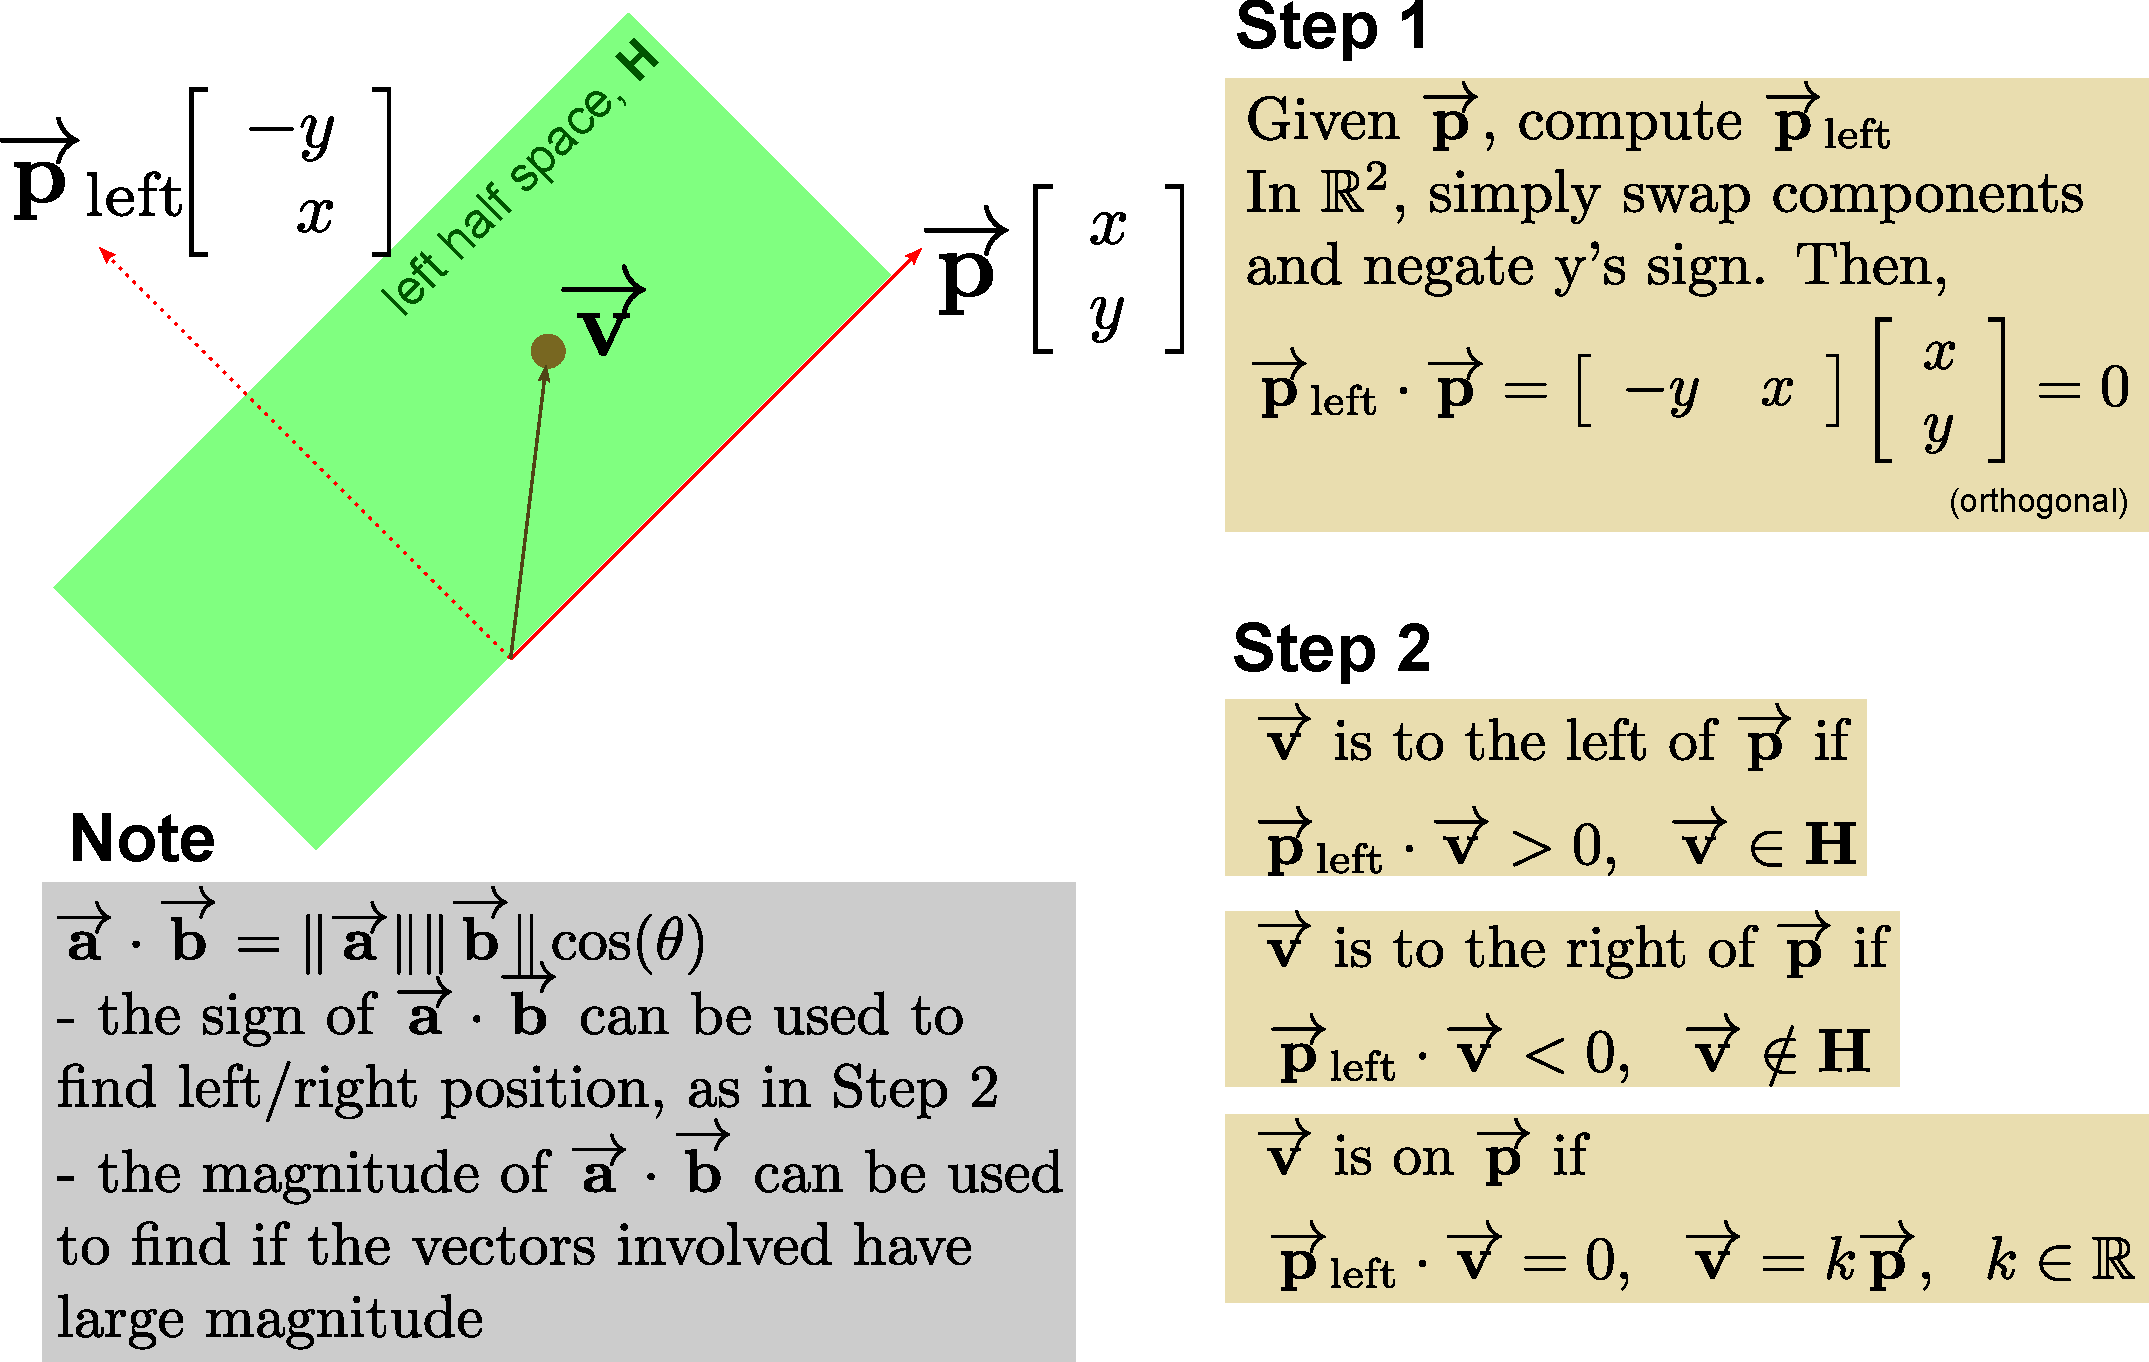
\includegraphics[width=0.75\textwidth]{figs/GRAPHICS_2D_left_turn.pdf}
								}
								\caption{Turning clockwise (left turn) in $\mathbb{R}^2$.}
								\label{fig:left_turn}
								\end{figure}


%\begin{equation}
%\begin{array}{llll}
%\mathbf{A} &= \left[\begin{array}{lll}a & b \\ c & d\\ \end{array}\right]\\
%&=\bigMatrixTwo
%\end{array}
%\end{equation}

where temporary variables $p, q, r, s$ are computed from angles $\theta$ and $\phi$ using,

\begin{equation*}
\begin{array}{llll}
\mathrm{ccc} &= \cos(\theta) \cos^2(\phi)\\
\mathrm{ccs} &= \cos(\theta) \cos(\phi) \sin(\phi)\\
\mathrm{css} &= \cos(\theta) \sin^2(\phi)\\
\mathrm{scc} &= \sin(\theta) \cos^2(\phi) \\
\mathrm{scs} &= \sin(\theta) \cos(\phi) \sin(\phi)\\
\mathrm{sss} &= \sin(\theta) \sin^2(\phi)\\
p   &=  \mathrm{css} - \mathrm{scs}\\
q   &=  \mathrm{ccc} + \mathrm{scs}\\
r   &= \mathrm{ccs} + \mathrm{sss}\\
s   &=  \mathrm{ccs} - \mathrm{scc}\\
\end{array}
\end{equation*}

The code for this step is given in Listing~\ref{lst:UTIL_2D_affine_tllpxy_to_abcdxy}.

								\begin{figure}[t]
								\centering
								\subfigure[User defined bounding box and feature points.]{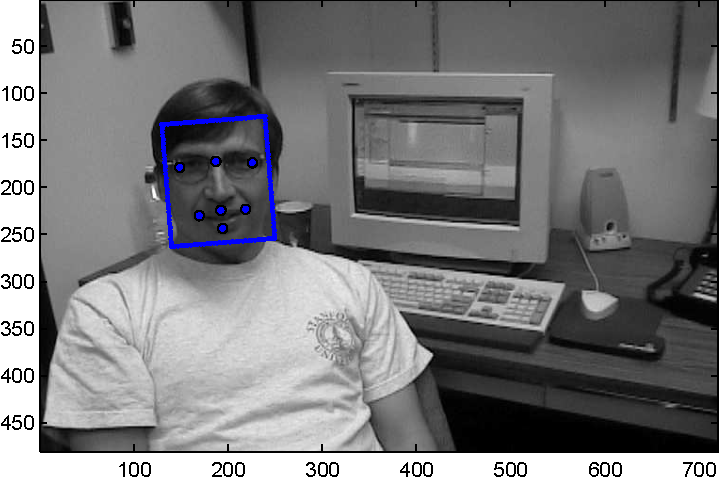
\includegraphics[width=0.65\textwidth]{figs/dataset_Dudek_with_feature_points_00001.pdf}}\\
								\subfigure[Desired output.]{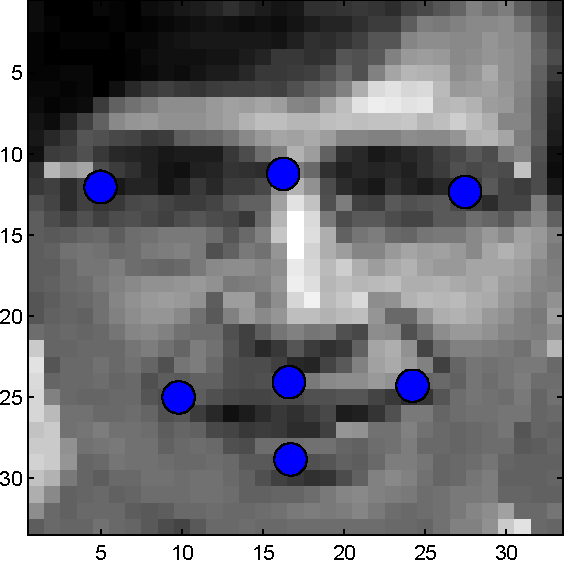
\includegraphics[width=0.25\textwidth]{figs/dataset_Dudek_desired_00001.pdf}}
								\caption{The goal is to scale and warp a user defined object of interest and corresponding feature points to an upright position.}
								\label{Fig:overall}
								\end{figure}



For our experiments, consider Figure~\ref{Fig:overall}.  The goal is to scale and warp a user defined object of interest and corresponding feature points to an upright position.  To achieve our goal, we design 2 experiments.  The goal of the first experiment is to warp and scale the actual image and the goal of the second experiment is to warp and scale the feature points.

Before we explain the experiments in detail, we discuss the overall idea.  Ideally, we could apply an inverse affine transform and be done with it.  There is one challenge though.  We do not know the pixel coordinates of every point inside the bounding region.  To deal with this, we design experiment 1 in which we take a rectangular grid whose coordinates we know, warp it using our affine parameters to cover the object of interest, interpolate image intensities on those points to create an upright scaled output image.  For the feature points, we do know their pixel coordinates and so in experiment 2, we straight away apply the inverse affine transform to compute their new positions in the output image.  So, in summary,

								\begin{figure}[t]
								\centering
								\fbox{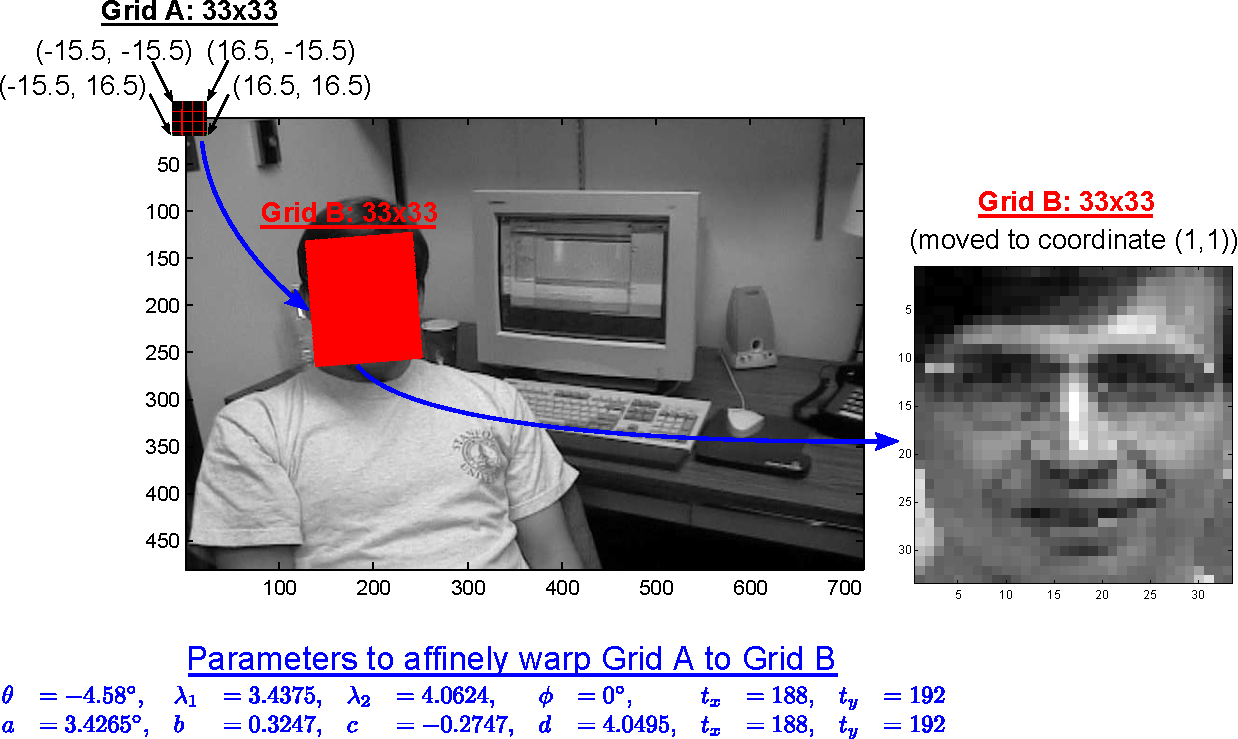
\includegraphics[width=0.85\textwidth]{figs/dataset_Dudek_00001_forwardAffine.pdf}}
								\caption{Experiment 1, Dudek dataset, frame 1, application of the forward affine transform.  In this experiment, we warp an arbitrary zero-centered grid to a grid covering the object of interest.  The dimensions of the object of interest, the face, are 110x130 (width x height).  The dimensions of the warped output grid are 33x33.  Notice that the density of grid points is greater in the horizontal direction.}
								\label{Fig:affine_warping}
								\end{figure}



\begin{enumerate}
\item Experiment 1: Forward affine transform to extract object of interest from original image
\begin{enumerate}
\item Warp user-defined grid using affine-parameter initialization to sample object of interest
\item Interpolate pixel intensities at warped grid-points.
\end{enumerate}
\item Experiment 2: Inverse affine transform to warp feature points on original image to warped image
\end{enumerate}


Before explaining these experiments in detail, we take a brief digression to explain how to compute affine parameters of the object of interest.

The source code for all these steps is given in Listing~\ref{lst:demo_UTIL_2D_coordinateAffineWarping_and_IntensityInterpolation}.

%------------------------------------------------------------
\subsection{Computing affine parameters of manually initialized object}
%------------------------------------------------------------
An object of interest in an image can be manually specified by drawing a bounding box around it, and then rotating the bounding box so that it reasonably encloses the object.  This step is relatively straightforward to do in standard image processing software.  In most cases, this rigid representation, as opposed to an affine representation, will suffice to reasonably enclose the object of interest for the purposes of initialization.  This requires 5 parameters for complete specification:

\begin{enumerate}
\item $t_x$, bounding box center x coordinate
\item $t_y$, bounding box center y coordinate
\item $w$, width of bounding box
\item $h$, height of bounding box
\item $\theta$, rotation angle of bounding box in radians.  In the cartesian coordinate system, a positive $\theta$ corresponds to counter-clockwise direction.  This can be verified quickly since a $90^{\circ}$ left turn for a vector $(x,y)^T$ in $\mathbb{R}^2$ is given by $(-y,x)^T$.  This is obtained using,

								\begin{figure}[t]
								\centering
								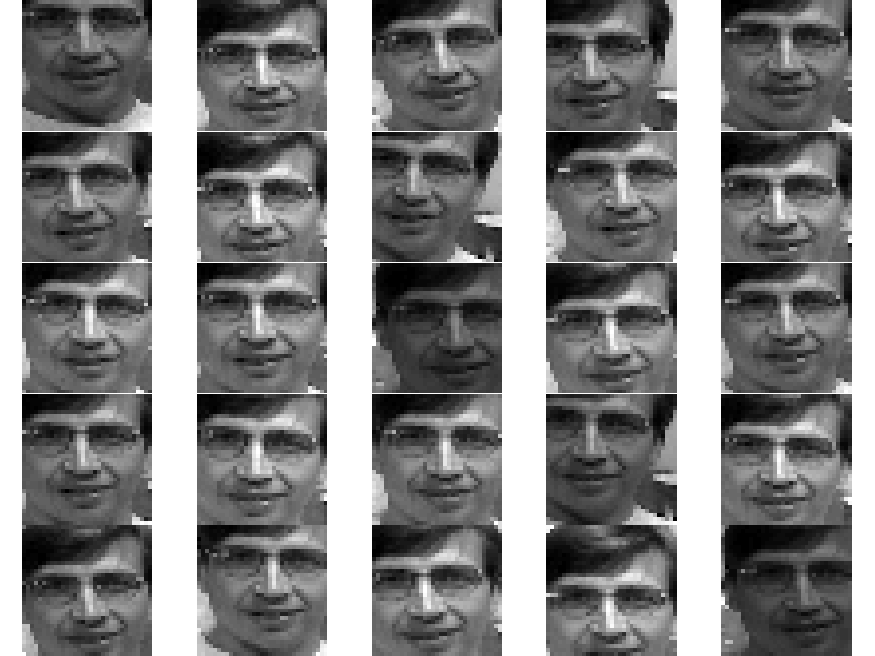
\includegraphics[width=0.65\textwidth]{figs/affineCandidates.pdf}
								\caption{Different affine parameters will produce different 33x33 outputs.}
								\label{Fig:affine_candidates}
								\end{figure}
\begin{equation}
\left[\begin{array}{ccc}
-y 
\\ 
x
\end{array}
\right]=
\left[
\begin{array}{rrr}
\cos(90^{\circ}) & -\sin(90^{\circ}) \\
\sin(90^{\circ}) & \cos(90^{\circ})
\end{array}
\right]
\left[\begin{array}{ccc}
x 
\\ 
y
\end{array}
\right]
\end{equation}

								\begin{figure}[t]
								\centering
								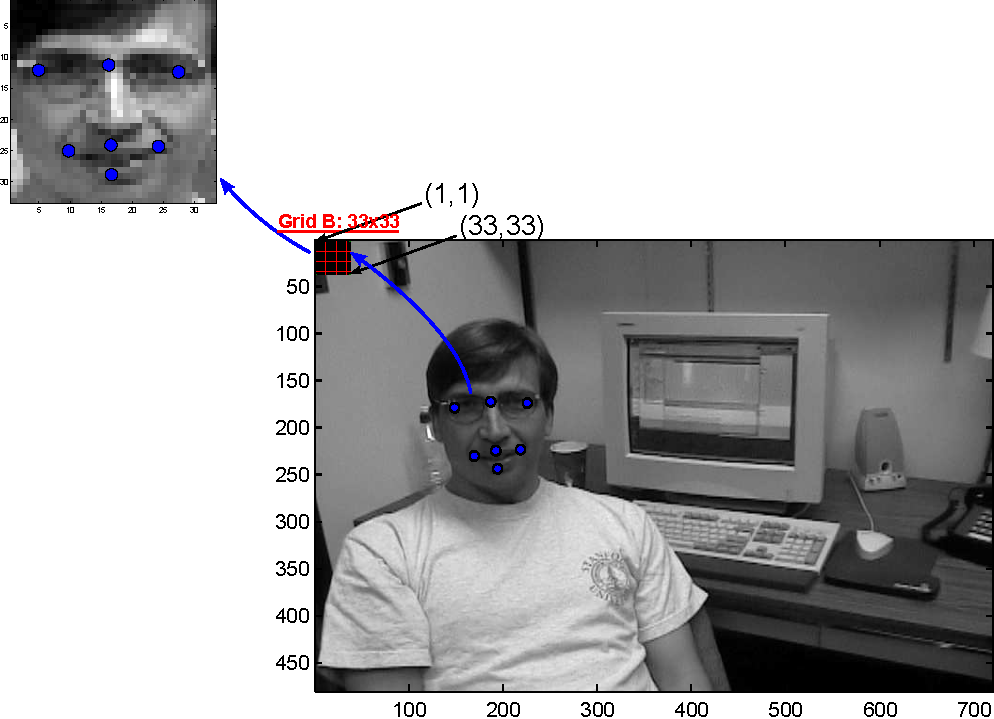
\includegraphics[width=0.75\textwidth]{figs/dataset_Dudek_00001_inverseAffine.pdf}
								\caption{Experiment 2, Dudek dataset, frame 1, application of inverse affine transform.  In this experiment, we apply the inverse affine transform to warp a set of given feature points and place them on Grid B from Figure~\ref{Fig:affine_warping}.}
								\label{fig:original_feature_points}
								\end{figure}


The term "left turn" is commonly used in computer graphics.  In  $\mathbb{R}^2$, it corresponds to a counter-clockwise rotation.  In images, where the $y$ coordinate normally decreases vertically downwards, a left turn is given by $(y,-x)^T$.  Notice that $(x,y)^T(-y,x) = (x,y)^T(y,-x) = 0$, and therefore both $ (-y,x)^T$ and $(y,-x)^T$ are orthogonal to $(x,y)^T$.  See Figure~\ref{fig:left_turn} for a graphical representation.
\end{enumerate}

As an example, consider Figure~\ref{Fig:affine_warping}.  We are interested in segmenting the face.  The initial parameters are: $t_x=188, t_y=192, w=110, h=130, \theta=-4.58^\circ$.  Note that we specify angles in radians.  $\theta$ is written here in degrees for clarity.  Moreover, notice that the bounding box is rotated in the counter-clockwise direction.  Since the y axis increases downwards, $\theta$ is negative.

Once we have an initial rigid representation of the object of interest, we can transform this representation into an affine representation.  Since the affine representation allows for scaling, we can scale the object and obtain its segmentation in scaled form.  For instance, in Figure~\ref{Fig:affine_warping}, the dimensions of the object of interest are 110x130.  However, for computational efficiency, we want the dimensions to be 33x33.  The affine parameters then become $\theta=-4.58^\circ, \lambda_1=110/32=3.4375, \lambda_2=130/32=4.0625, \phi=0^\circ, t_x=188, t_y=192$.  \footnote{Notice that we have divided by 32 instead of 33.  The reason is that the grid used in~\cite{2008_JNL_subspaceTRK_Ross} is 32x32 and they have accordingly used a divisor of 32.  In our case, for RVQ we require an odd dimensional grid due to the way the closed source codebook encoding software, gen.exe is setup.  Therefore, we pick a 33x33 grid.  Not changing the divisor to 33 was an oversight but this omission is expected to have minimal effect on results.}


%----------------------------------
\subsection{Experiment 1: Forward affine transform}
%----------------------------------
In this experiment, our goal is to extract an object of interest from an original image, scale it and make it upright.  We start with an arbitrary zero-centered grid, grid A as shown in Figure~\ref{Fig:affine_candidates}.  The forward affine transform is applied to this grid so that it covers the object of interest and is now called grid B.  Note that the dimensions of grid B are also 33x33.  Grid B is now placed at coordinates (1,1) so that its coordinates go from 1 to 33 in the horizontal direction and 1 to 33 in the vertical direction.  Note that this grid now samples the object of interest.  This grid is then placed at the origin as shown in Figure~\ref{fig:original_feature_points}.  

\subsubsection{Warp user-defined grid}
%------------------------------------------------------------
In this step, the affine parameters $(\theta, \lambda_1, \lambda_2, \phi, t_x, t_y)$ computed above are changed to $(a, b, c, d, t_x, t_y)$ using Equation~\ref{Eqn:tllpxy_to_abcdxy}.  Affine matrix $\mathbf{H}_A$ is formed using Equation~\ref{Eqn:top_level}.  A reference $w$ x $h$ = 33x33 grid centered on the origin is transformed using these affine coordinates to a 33x33 grid centerd on the object of interest using the affine transformation also given in Equation~\ref{Eqn:top_level}.  This can be seen in Figure~\ref{Fig:affine_warping}.

\subsubsection{Interpolate pixel intensities}
%------------------------------------------------------------
The final step is to read off the pixel intensity values at the affinely warped grid obtained in the step above.  Most of these grid points will not have integer values.  Rounding to integer values will create artefacts.  Some form of interpolation will be required to read sub-pixel intensities.  In our experiments, we use bilinear interpolation. 

As a sidenote, we show the effects of applying different affine transform parameters in Figure~\ref{Fig:affine_candidates}.  This can be useful for instance to generate samples in the particle filter.


%----------------------------------
\subsection{Experiment 2, Inverse affine transform}
%----------------------------------
Now, feature points on the original figure are inverse-affine-transformed and superimposed on grid B.  A feature point with coordinates $(X,Y)$ can be inverse affine mapped to $(x,y)$ using

\begin{equation}
\left[\begin{array}{ccc}
x 
\\ 
y
\end{array}
\right]
=
\left[\begin{array}{ccc}
a & b\\ 
c & d
\end{array}
\right]^{-1}
\left[\begin{array}{ccc}
X - t_x  
\\ 
Y - t_y
\end{array}
\right]
\end{equation}

For our example, the initial feature points are 

\begin{equation*}
\left[\begin{array}{ccc}
X  
\\ 
Y
\end{array}
\right]=
\left[
\begin{array}{cccccccc}
148.9306 & 187.2747 & 226.0674 & 169.6408 & 192.6433 & 218.8531 & 194.5372\\
179.0198 & 172.5994 & 174.0397 & 230.2172 & 224.5582 & 223.3328 & 243.8089\\
\end{array}
\right]
\end{equation*}

Applying the inverse affine transform yields

\begin{equation*}
\left[\begin{array}{ccc}
x  
\\ 
y
\end{array}
\right]=
\left[
\begin{array}{rrrrrrrrrrr}
  -11.0275 &   0.2407 &  11.4563 &  -6.2122  &  0.5896 &   8.2183 &   0.6912\\
   -3.9534  & -4.7745  & -3.6580  &  9.0161  &  8.0800  &  8.2949  & 12.8408
\end{array}
\right]
\end{equation*}


Notice that the inverse mapped feature points are zero-centered.  We add $(w/2, h/2)$ so that these warped feature points correctly align with grid B whose first x and y coordinate is at (1,1).\footnote{This uses Matlab notation rather than C++ notation where the first x and y coordinates are at (0,0).}  This gives,

\begin{equation*}
\left[\begin{array}{ccc}
x  
\\ 
y
\end{array}
\right]=
\left[
\begin{array}{rrrrrrrrrrr}
   5.4725  & 16.7407 &  27.9563  & 10.2878  & 17.0896 &  24.7183  & 17.1912 \\
   12.5466 &  11.7255 &  12.8420 &   25.5161 &  24.5800  & 24.7949 &   29.3408
\end{array}
\right]
\end{equation*}

These points are plotted in Figure~\ref{fig:original_feature_points}.


Figure~\ref{Fig:affine_warping} shows the result of affine warping to compute warped grid points and bilinear interpolation to compute pixel intensities on those warped grid points to produce an upright scaled image.  We see that the affine region of interest accurately samples the object of interest and minimizes inclusion of background pixels.  Also, bilinear interpolation produces an accurate representation of the target of interest.  The original feature points are also correctly warped and overlaid on the output image.


Affine warping is an effective way of extracting an object of interest and associated feature points from a given image.  The affine representation is rich enough to bound many objects of interest while minimizing inclusion of background pixels.


%=======================		
\section{Model 4: Motion model}
%=======================		
The motion model is a mathematical representation of the real or expected motion of the target of interest.  Since tracking is in general an ill-posed problem, it is common to make assumptions about the motion to simplify motion modeling.  Common assumptions such as stationary camera, coherent motion etc. are discussed in Chapter~\ref{chap_Tracking_methods}.

In this work, we make two assumptions about the target motion:

\begin{itemize}
\item \underline{Coherent motion}.  We assume that each part of the target moves together.  The target can deform and warp but it does not break up into individual parts.
\item \underline{Can be modeled with a gaussian distribution with fixed variance}.  We assume that the motion is brownian and can be modeled with a gaussian distrubution with a fixed variance.  
\end{itemize}

An advantage of not having an explicit motion model is that arbitrary camera and target motion are allowed.  A disadvantage of this approach in the context of the particle filter is that particles need to be evaluated all around the current target position, rather than only around the projected target position.  We are therefore unable to take advantage of the reduced spatial search-space that comes with a deterministic motion model.  

Two of the six components of the state vector $\mathbf{X}$ deal with the motion model.  These are the $x$ and $y$ coordinates of the target.  These are modeled as independent gaussian random variables with fixed variance $\sigma_x^2, \sigma_y^2$,

\begin{align*}
p(x_t|x_{t-1}) &= \mathcal{N}(x_{t-1}, \sigma_x^2) \\
p(y_t|y_{t-1}) &= \mathcal{N}(y_{t-1}, \sigma_y^2) \\
\end{align*}

\newpage
At every frame, we try to estimate a state vector $\mathbf{X}$ in $R^6$.  Two components of this vector, the target coordinates are related to the motion model and the remaining four are related to the affine deformation allowed by the representation model.  To keep our models as general as possible, all 6 components of the state are modeled as Gaussian random variables but with known variance.  However, in order to simplify sampling from the joint density, it is possible to use certain relaxation criteria such as Markovian dependence, or complete independence.  We choose the latter to make the sampling process in the inference model somewhat more straightforward.

Our motion model then consists of 6 uncorrelated gaussian densities. 
The target motion is therefore represented not in analytic form but as a 6x6 diagonal covariance matrix $\Sigma_X$ centered at the target position $\mathbf{X}_{t-1}$ in the previous frame.  The elements on the diagonal represent variances of affine parameters, $\sigma_x^2, \sigma_y^2, \sigma_\theta^2, \sigma_s^2, \sigma_\alpha^2, \sigma_\phi^2$.   


Several Gaussian distributions are used to handle these changes.  One distribution each is used to handle arbitrary translation in the horizontal direction, vertical direction, scale, rotation.  At every time step, predicted values are sampled from these distributions.  Each predicted value is warped to a standard window size and tested against the existing model.  The predicted value closest to the current model is selected as the next estimate and is used to update the model.  In PCA, the model is the eigenvectors, in RVQ, it's the stage codevectors and in TSVQ, it's the terminal codevectors.  

In this work, we model the object motion by an affine image warp.  The state at time $t$ consists of 6 affine transformation parameters: $x_t,  y_t, \theta_t, s_t, \alpha_t$, and $\phi_t$.




%=======================		
\section{Model 5: Inference model}
%=======================	
Track targets under the following conditions:

\begin{itemize}
\item Target dynamics are non-linear
\item Target dynamics are non-Gaussian
\item Online processing is required
\end{itemize}


%-----------------------------------------------------
\subsection{Introduction}
%-----------------------------------------------------
In the state-space approach to time series modeling, the focus is on the \emph{state vector} and its transition from state to state.  In tracking applications, the state vector could correspond to target dynamics.  In economic systems, the state vector could be composed of quantities such as inflation rates, currency exchange rates, inflation, etc.  In weather forecasting, the state vector could be based on hurricane speed, direction and strength.  It is clear that a large range of applications can be modeled using this approach.  However, in most cases, it is difficult to accurately estimate the states.  Noise induced by natural phenomena or erroneous observation can corrupt measurement of the state vector.  A noisy \emph{measurement vector} therefore relates observations to states.

In many cases, the state vector evolution can be modeled as a linear system,

\begin{align}
\mathbf{x}[k] &= \mathbf{A}\mathbf{x}[k-1] +  \mathbf{B}\mathbf{u}[k]\\
\mathbf{z}[k] &= \mathbf{A}\mathbf{x}[k] +  \mathbf{v}[k]\\
\end{align}

In such cases, One such example is given in Figure~\ref{TRK_overviewDiagram}.  

								\begin{figure}[t]
								\center
								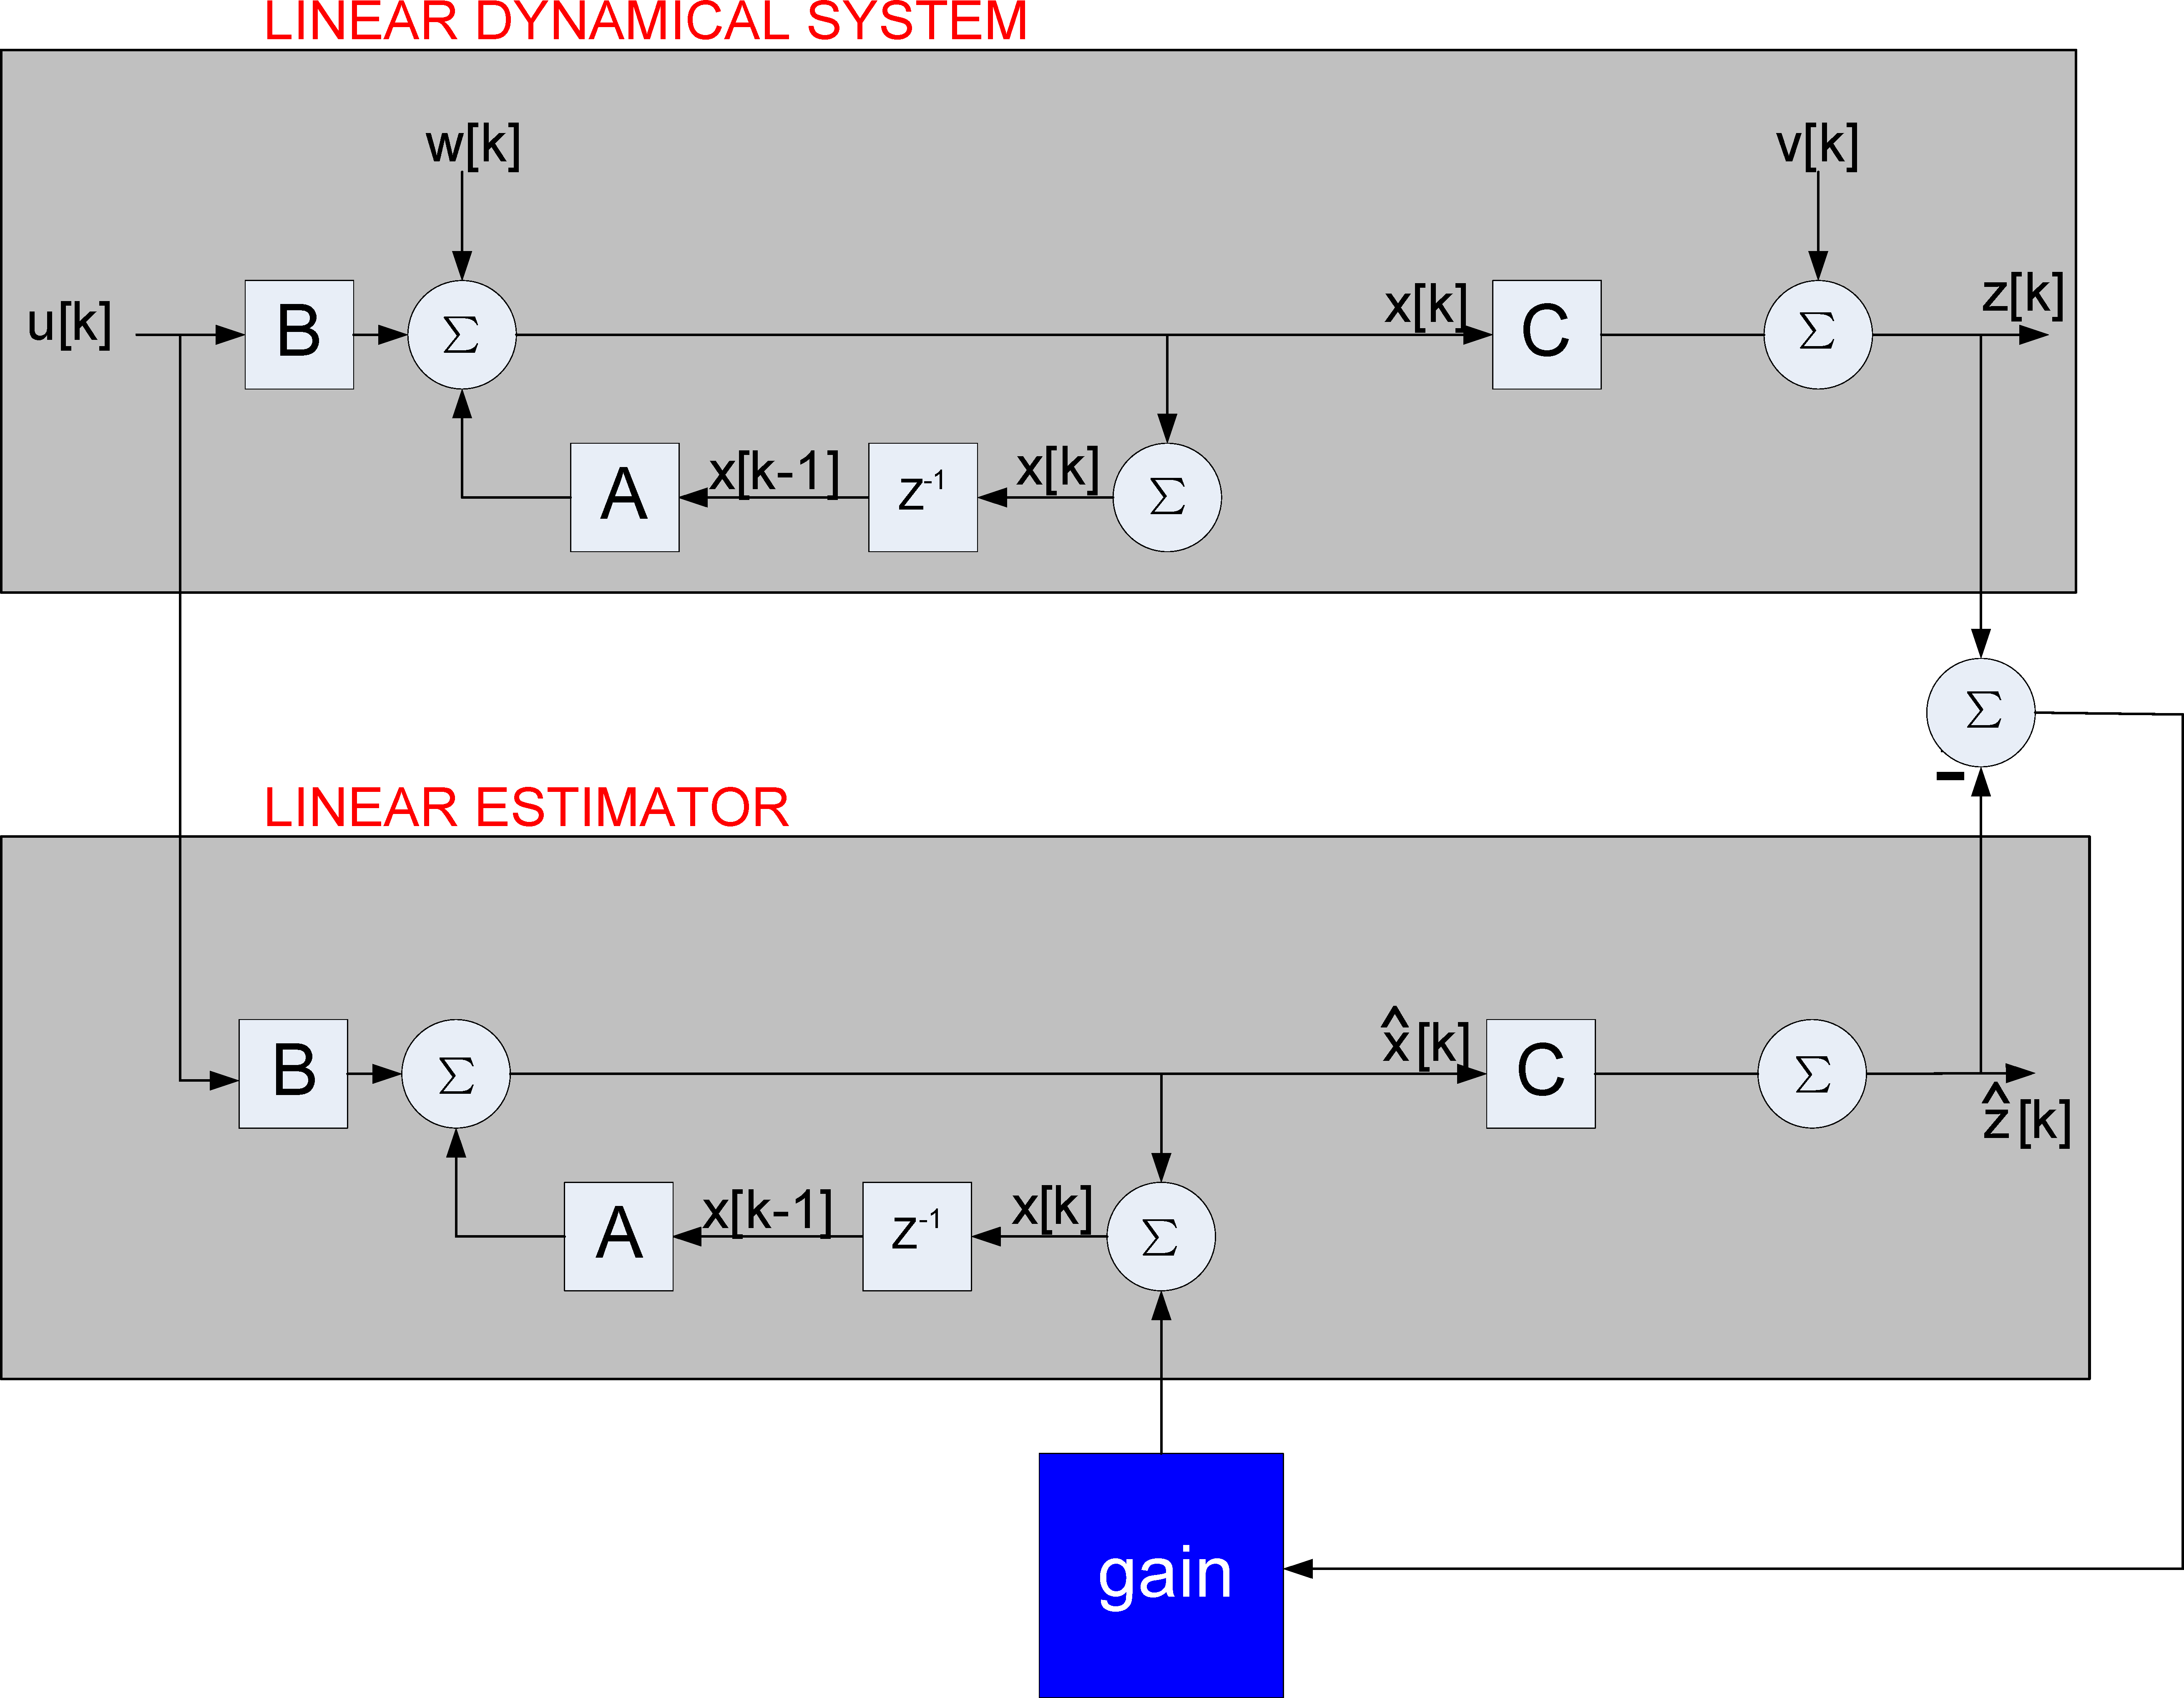
\includegraphics[width=1.0\textwidth]{figs/TRK_LinearEstimator_blockDiagram.pdf}
								\caption{Linear estimator.}
								\label{TRK_overviewDiagram}
								\end{figure}


The inference model in this work is based on a sequential Monte Carlo (SMC) filter, the particle filter.  The particle filter has been discussed in Chapter~\ref{chap_TRK}.  Almost all particle filters are based on the sequential importance sampling (SIS) algorithm, including the sampling importance resampling (SIR) filter, auxiliary sampling importance resampling (ASIR) filter and the regularized particle filter (RPF).  The basic difference between these algorithms is the choice of \emph{importance sampling density} and/or modification of the resampling step~\cite{2002_JNL_PF_Arulampalam}.  

In this work, we use the basic SIS algorithm.  It is essentially the same as the SIR filter except that there is no resampling step.  However, like the SIR filter, we use the prior density as the importance sampling density.  The weights on the posterior are computed using the appearance model for PCA, RVQ or TSVQ, depending on which of these algorithms is being used.  For RVQ for instance, the mean squared reconstruction error is used for the weighting.

A commonly used formulation for tracking is based on Bayesian estimation.  In this framework, target kinematics are modeled as the latent states of a time-dynamic system~\cite{2002_JNL_PF_Arulampalam}.  Time-dynamic systems are based on two models: (a) \emph{state prediction model}, ${f_t:R^D \times R^D \rightarrow R^D}$, describing state evolution, and (b) \emph{observation model}, ${h_t:R^N \times R^N \rightarrow R^N}$, relating observations to the states.  These models are described as,

\begin{align}
\mathbf{x}_t &= f_t(\mathbf{x}_{t-1}, \mathbf{v}_{t-1}) \notag\\
\mathbf{z}_t &= h_t(\mathbf{x}_t, \mathbf{n}_t)
\label{Eq:TDS}
\end{align}

$\mathbf{v} \in R^D$ is an independent, identically-distributed (IID) process noise sequence.  $\mathbf{n} \in R^N$ is an IID measurement noise sequence.  The goal is to find the estimate of the state $\mathbf{x}_t$ at time $t$, based on all observations $\mathbf{Z}_t={\{\mathbf{z}_i, i=1,...,T\}}$.   $\mathbf{z}_t$ is the observation vector at time $t$.  

At this point, it is interesting to place the process of tracking in the bigger picture of probabilistic graphical models, as shown in Figure~\ref{fig:TRK_big_picture}.  Mathematically, hidden Markov models (HMMs) can also be written using evolution and observation models even though the method was developed independently of time dynamic systems \cite{2007_BOOK_PRML_Bishop}.  

This two stage model lends itself well to Bayesian inference \cite{2002_JNL_PF_Arulampalam}.  The reason is that observations can be used as evidence to modulate the prior distribution on the states.  We can then infer the posterior distribution on the states using Bayes' Rule.  Mathematically, the Chapman Kolmogorov equation predicts the next state by combining information from the state prediction model $p(\mathbf{x}_t| \mathbf{x}_{t-1})$ and all previous observations $\mathbf{Z}_{t-1}$.  %This is given in Equation~\ref{Eqn:TRK_prediction}.

{%\Large
\begin{equation}
\begin{array}{lllllllll}
{\color{darkgreen}p(x_t|Z_{t-1})} &= \frac{p(x_t, Z_{t-1})}{p(Z_{t-1})}\\
&=\frac{\int p(x_t, x_{t-1}, Z_{t-1})dx_{t-1}}{p(Z_{t-1})}\\
&=\frac{\int {\color{Cyan}p(x_t|x_{t-1}, Z_{t-1})}p(x_{t-1},Z_{t-1})dx_{t-1}}{p(Z_{t-1})}\\
&=\frac{\int {\color{Cyan}p(x_t|x_{t-1})}{\color{red}p(x_{t-1}|Z_{t-1})}p(Z_{t-1})dx_{t-1}}{p(Z_{t-1})}\\
&=\int {\color{Cyan}p(x_t|x_{t-1})}{\color{red}p(x_{t-1}|Z_{t-1})}dx_{t-1}
\end{array}
\label{Eqn:TRK_prediction}
\end{equation}
}


%\begin{equation}
%p(x_k|\textbf{Z}_{k-1})=
%\int{p(\mathbf{x}_k| \mathbf{x}_{k-1})p(\mathbf{x}_{k-1}|\mathbf{Z}_{k-1})}d\mathbf{x}_{k-1}
%\label{eq:ChapmanKolmogorov}
%\end{equation}  

In the second step, the observation $\mathbf{z}_t$ at time $t$ and the predicted state $\mathbf{x}_t$ can be used to compute the posterior estimate of the state $\mathbf{x}_t$ using %Equation~\ref{Eqn:TRK_update}.


{%\large
\begin{equation}
\begin{array}{lllllllll}
{\color{red}p(x_t | Z_t)} &= \frac{p(x_t, Z_t)}{p(Z_t)}\\
&= \frac{p(x_t, z_t, Z_{t-1})}{p(z_t, Z_{t-1})}\\
&= \frac{{\color{blue}p(z_t|x_t,Z_{t-1})}p(x_t, Z_{t-1})}{p(z_t|Z_{t-1})p(Z_{t-1})}\\
&= \frac{{\color{blue}p(z_t|x_t)}{\color{darkgreen}p(x_t|Z_{t-1})}p(Z_{t-1})}{p(z_t|Z_{t-1})p(Z_{t-1})}\\
&= \frac{{\color{blue}p(z_t|x_t)}{\color{darkgreen}p(x_t|Z_{t-1})}}{\int{p(z_t|x_t){\color{darkgreen}p(x_t |Z_{t-1})}}dx_t}
\end{array}
\label{Eqn:TRK_update}
\end{equation}
}



%\begin{equation}
%p(\mathbf{x}_k|\textbf{Z}_k)	= \frac{p(\mathbf{z}_k|\mathbf{x}_k)p(\mathbf{x}_k |\textbf{Z}_{k-1})   }{p(\mathbf{z}_k| \textbf{Z}_{k-1})}
%\label{eq:posterior}			
%\end{equation}

Equations~\ref{Eqn:TRK_prediction} and~\ref{Eqn:TRK_update} form the optimal Bayesian solution for the recursive propagation of the posterior density.  This problem can be solved analytically using the closed-form Wiener-Kalman linear Minimum Mean Square Estimate (MMSE) in Gaussian noise \cite{1964_JNL_BayesianEstimation_Ho, 1993_BOOK_SSP_Kay}.  Non-analytical methods, such as grid-based methods, can be used if the state space is discrete and consists of a finite number of states.  For non-linear models, the Extended Kalman Filter (EKF) computes the Jacobian for a Taylor Series expansion of the system and observation models about the current state \cite{2005_Misc_KalmanFilterComparison_Orderud}.  Recently, the Unscented Kalman Filter (UKF) has been replacing the EKF in a wide range of applications.  The UKF, instead of explicitly computing the Jacobian, computes a set of points that capture the true mean and covariance of the prior.  When propagated through the non-linear system, these points capture the posterior mean and covariance \cite{1997_CNF_UKF_Julier}.  As a result, the UKF estimates the posterior mean and covariance accurately to at least the second-order Taylor Series expansion.  The EKF on the other hand achieves only first-order accuracy \cite{2004_CNF_SigmaPointKalman_Merwe, 2000_CNF_UKF_Wan}.  More recently, particle filters which use point mass representations for probability densities and are based on stochastic sampling have been introduced in the visual tracking literature \cite{1993_JNL_ParticleFilter_Gordon, 2001_JNL_PFjumpMarkov_Doucet}.  A primary difference between the UKF and the particle filter is that the former is based on deterministic sampling while the latter is based on stochastic sampling.  Particle filters offer an additional advantage of being able to handle arbitrary densities as shown in Figure~\ref{fig:particle_filter_multi_modal_density}.  However, since the particle filter uses non-parametric densities with no functional representations, its computations do not scale well as the dimensionality increases~\cite{2004_CNF_TrackingPeople_Zhao}.  

A variety of particle filters have now been introduced.   According to~\cite{2002_JNL_PF_Arulampalam}, sequential Monte Carlo (SMC) filtering has been called particle filtering~\cite{1999_CNF_PF_carpenter}, bootstrap filtering~\cite{1993_JNL_ParticleFilter_Gordon}, the condensation algorithm~\cite{1998_JNL_Condensation_IsardBlake}, interacting particle approximations~\cite{1999_JNL_PF_Crisan, 1999_BK_PF_Moral} and survival of the fittest~\cite{1995_CNF_PF_Kanazawa}.

  
%The particle filter formulation is generally similar to the method which is used for the Kalman Filter.  A prediction step is followed by an update step, which is followed by a prediction step, and so on.  The update equation at time $t$ for a state $x_t$ given all observations $z_T$ involves computing the posterior density $p(x_t | Z_t)$.  In this case, the posterior density factors into a likelihood at time $t$, $p(z_t|x_t)$ and a prior density, $p(x_t|Z_{t-1})$, 
%
%
%
%
%The prior density can be computed using the Chapman-Kolmogorov equation by introducing the nuisance parameter $x_{t-1}$,
%
%
%$p(x_t|x_{t-1})$ is computed using the motion model while $p(x_{t-1}|Z_{t-1})$ is the posterior density from the previous time step, $t-1$.
%
%
%Visual tracking in clutter is difficult using the Kalman filter since clutter can typically give rise to several competing observations which encourage a non-unimodal density and gaussian densities cannot represent simultaneous alternative hypotheses~\cite{1998_JNL_Condensation_IsardBlake}.  Moreover 


%However, currently, the most popular version is the SIR (Sampling Importance Resampling) filter \cite{2009_BOOK_PF_Doucet}.  The resampling step prevents the posterior from collapsing to a single point.  The steps involved in computing the solution to this filter are summarized below:

%\begin{itemize}
%\item \textbf{Sampling with replacement.}  This step is carried out to guarantee that the algorithm runs within given computational resources.  $N$ samples are chosen from the set $\mathbf{s}_{k-1}^n$, each element being chosen with probability $\pi_{k-1}^n$.  %a sampling with replacement st from $p(\mathbf{x}_k | \mathbf{x}_{k-1})$
%\item Calculate particle weights from the likelihood, $\mathbf{w}_k = p(\mathbf{z}_k|\mathbf{x}_k)$
%\item Calculate the posterior ($p(\mathbf{x}_k | \mathbf{x}_{k-1})$.  First normalize weights.  Then resample using normalized-weights and sampled-prior. 
%\end{itemize}
The density to be resampled is called the test density.


								\begin{figure}[t]
								\centering
								\subfigure[Reference (uniform) density and test PDF.]{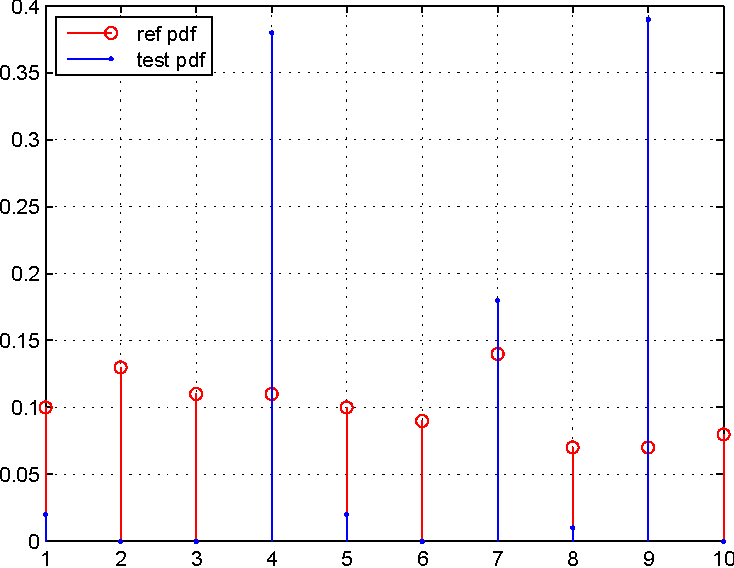
\includegraphics[width=0.4\textwidth]{figs/particle_filter_pdfs.pdf}}
								\subfigure[Comparing CDFs.]{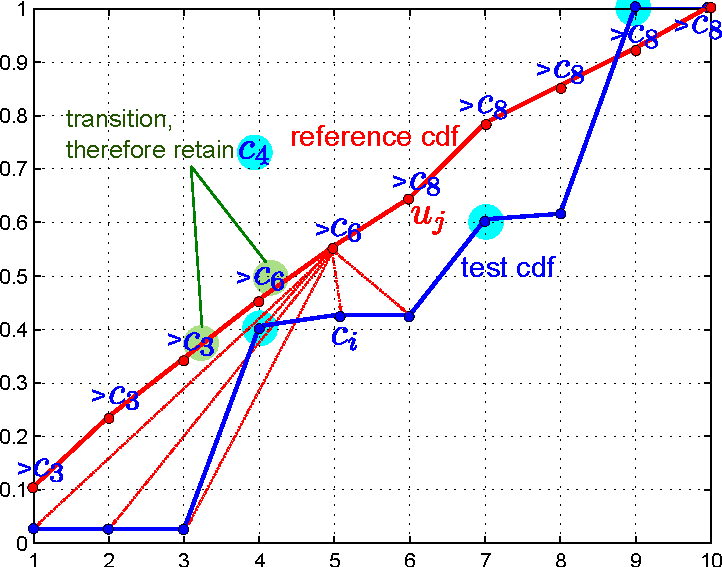
\includegraphics[width=0.4\textwidth]{figs/particle_filter_resampling.pdf}}
								\subfigure[Particles 4, 7 and 9 are picked repeatedly since they have higher weight.]{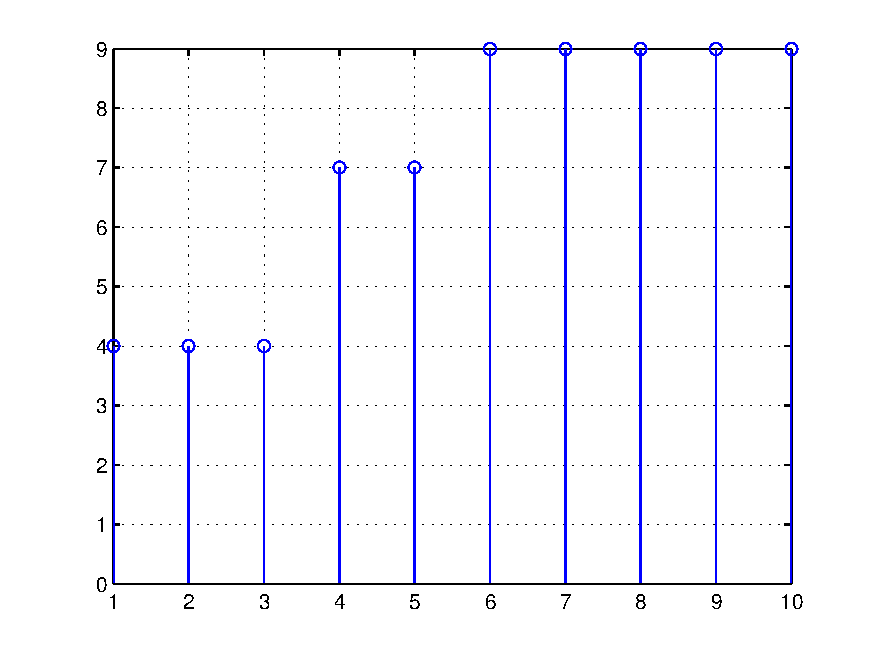
\includegraphics[width=0.45\textwidth]{figs/particle_filter_particles.pdf}}
								\subfigure[Resampled PDF.]{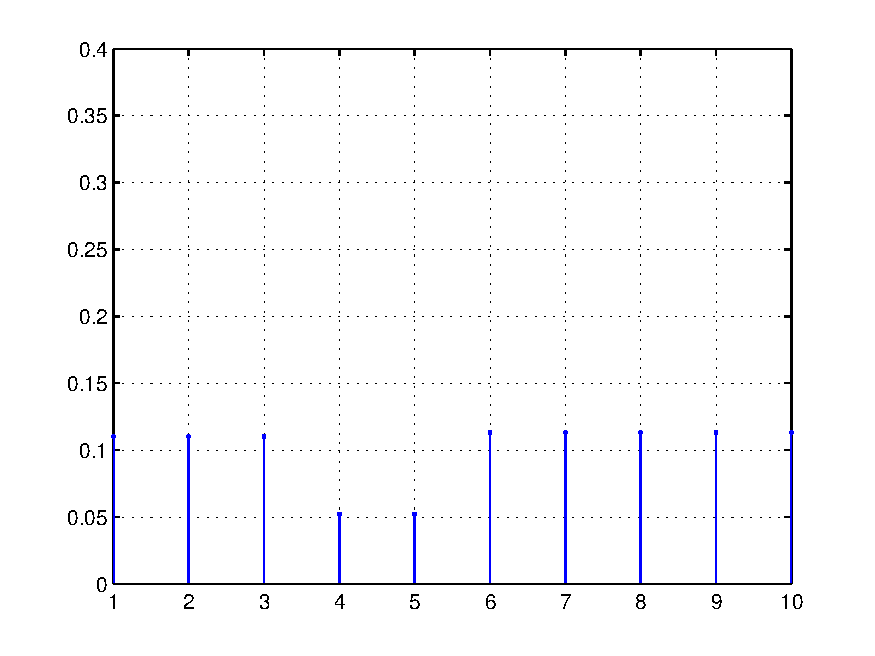
\includegraphics[width=0.45\textwidth]{figs/particle_filter_resampled_density.pdf}}
								\caption{Particle filter, resampling.  Source code for this is given in Listing~\ref{lst:main_TRK_particle_filter_resampling} and~\ref{lst:TRK_particle_filter_resampling}}.   
								\label{fig:particle_filter_resampling}
								\end{figure}
								

\subsection{Resampling}
Samples are generated from a uniform density.  The CDF of this reference density is then compared with the CDF of the test density.  This is shown in Figure~\ref{fig:particle_filter_resampling}.  Each value of the reference density is compared with values of the test density. 
	
The inference model in this work is based on a sequential Monte Carlo (SMC) filter, the particle filter.  The particle filter has been discussed in Chapter~\ref{chap_Tracking_methods}.  Almost all particle filters are based on the sequential importance sampling (SIS) algorithm, including the sampling importance resampling (SIR) filter, auxiliary sampling importance resampling (ASIR) filter and the regularized particle filter (RPF).  The basic difference between these algorithms is the choice of \emph{importance sampling density} and/or modification of the resampling step~\cite{2002_JNL_PF_Arulampalam}.  

In this work, we use the basic SIS algorithm.  It is essentially the same as the SIR filter except that there is no resampling step.  However, like the SIR filter, we use the prior density as the importance sampling density.  The weights on the posterior are computed using the appearance model for PCA, RVQ or TSVQ, depending on which of these algorithms is being used.  For RVQ for instance, the mean squared reconstruction error is used for the weighting.

The number of particles used is $N_p=600$.  Each particle represents the point mass density of a vector $\mathbf{X}$ in $R^6$ corresponding to the 6 parameters required for an affine deformation.

\cite{1992_JNL_MCMC_Carlin}


\begin{table}[t]
\footnotesize
\begin{tabular}{p{0.6in}|p{0.6in}p{0.6in}p{0.4in}p{0.4in}cccccc}
Dataset 		&Scenario	     &\parbox[c]{0.4in}{\center Time of \\day} 	&\parbox[c]{0.26in}{\center Target of \\interest}  &\parbox{0.3in}{\center Rigid \\target} 	&\parbox{0.4in}{\center Lighting change 1-5 \\(5 most severe)}  	&\parbox{0.5in}{\center Structured \\noise} 	&\parbox{0.4in}{\center Camera \\motion} 	&\parbox{0.3in}{\center Pose \\change} 	&\parbox{0.45in}{\center Expression \\change} 	&\parbox{0.3in}{\center Temporary \\occlusion} 	\\\hline
Dudek 			&Indoors 	     &N/A 			&human 					&no 	&1 	&yes 	&yes 	&yes 	&yes 	&yes 		\\\hline
davidin300 	&Indoors		&N/A			&human					&no	&2	&yes	&yes	&yes	&yes	&no		\\\hline
sylv				&Indoors		&N/A			&toy						&yes	&4	&no	&yes	&yes	&N/A	&no		\\\hline
trellis70	 		&Outdoors 		&day, dark		&human					&no	&5	&no	&yes	&yes	&yes	&no		\\\hline
fish				&Indoors		&N/A			&object					&yes	&4	&no	&yes	&no	&N/A	&no		\\\hline
car4			&Outdoors 		&day, sunny	&vehicle					&yes	&3	&no	&yes	&yes	&N/A	&no		\\\hline
car11			&Outdoors		&night			&vehicle					&yes	&4	&no	&yes	&yes	&N/A	&no		\\\hline
\end{tabular}
\caption{Datasets used for RVQ tracking.}
\label{Tab:datasets_used}
\end{table}

In this report, our goal is to present tracking error results for our 6 different trackers, PCA-based, TSVQ-based and 4 RVQ-based trackers, maxP, RofE, nulE, and monR.


								\begin{figure}[t]
								\centering
								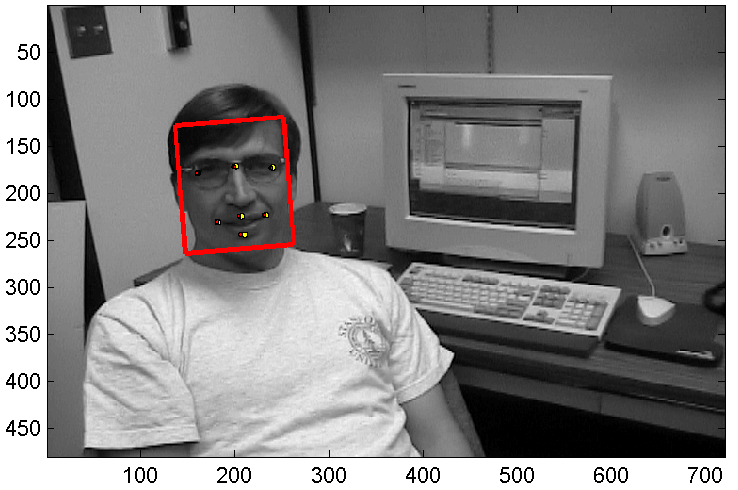
\includegraphics[width=0.7\textwidth]{thesis/results_pca__trk_dudek_0007.png}
								\caption{Computing tracking error.  The larger yellow circles indicate ground truth feature points.  The smaller red circles indicate estimated feature points.  Tracking error is computed using the rms error between the ground truth feature points and the estimated feature points.  In this particular frame, the tracking error is 2.57.}
								\label{fig:results_pca__trk_dudek_0007}
								\end{figure}

We have previously described our 5-component tracker comprising appearance, observation, representation, motion and inference models.  All 6 trackers share exactly the same representation, motion and inference models.  However, each has its own appearance and observation models.

All trackers were run on 6 publicly available datasets, Dudek, davidin300, sylv, fish, car4 and car11.  See Figure~\ref{fig:trk_sequences} in Appendix~\ref{App:dataset_snapshots} for snapshots of images in each dataset at 100 image intervals.  These datasets can be downloaded from~\cite{2008_JNL_subspaceTRK_Ross}.  Tracking error was measured on each of these datasets using the error between ground truth feature points and estimated feature points as shown in Figure~\ref{fig:results_pca__trk_dudek_0007} for the Dudek sequence.

								\begin{figure}[t]
								\centering
								\begin{tabular}{|l|c|c|c|c|c|c|}
\hline
&\textbf{PCA}&\textbf{TSVQ}&\textbf{maxP}&\textbf{RofE}&\textbf{nulE}&\textbf{monR}\\\hline
\textbf{Dudek}&7.44&8.62&7.78&7.11&7.97&8.73\\\hline
\textbf{davidin300}&4.60&5.93&4.47&5.74&4.63&4.15\\\hline
\textbf{sylv}&4.34&4.61&4.00&4.12&4.74&4.31\\\hline
\textbf{fish}&2.17&4.59&2.78&2.73&2.48&2.89\\\hline
\textbf{car4}&4.60&5.11&4.67&4.93&5.28&4.71\\\hline
\textbf{car11}&2.13&2.21&2.17&2.33&2.52&2.47\\\hline
\textbf{ \% best}&50.00&0.00&16.67&16.67&0.00&16.67\\\hline
\end{tabular}

								\subfigure[Best tracking error for each algorithm.]{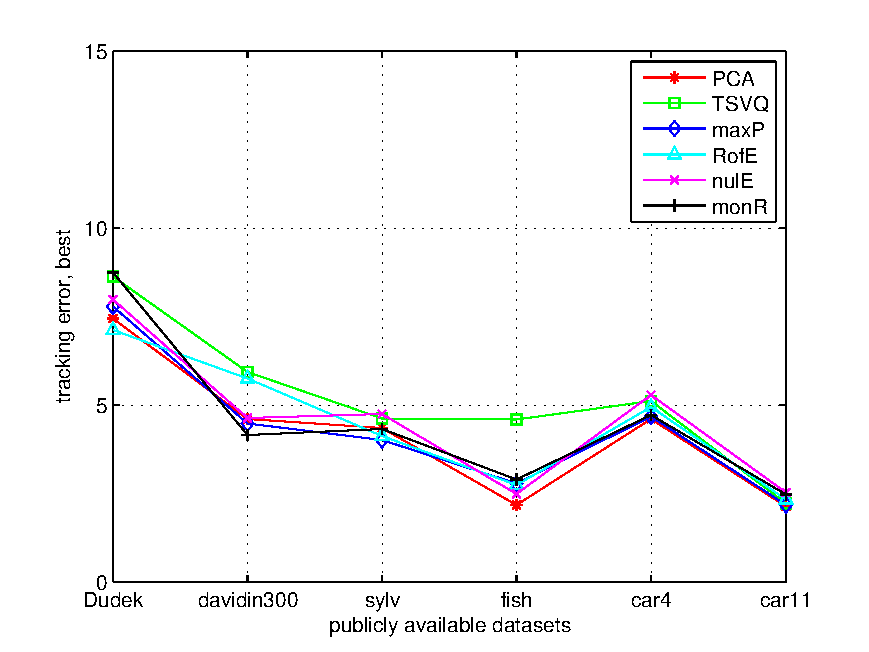
\includegraphics[width=0.47\textwidth]{thesis/results_final_1a_best.pdf}\label{fig:results_final_1a_best}}
								\subfigure[\%age of datasets over which best tracking error is achieved over all parameters.]{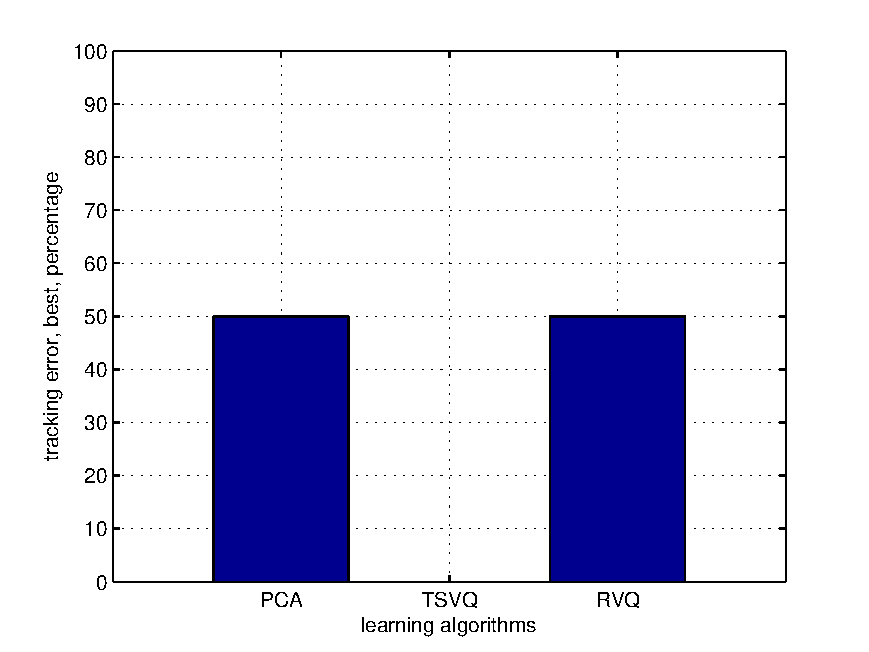
\includegraphics[width=0.47\textwidth]{thesis/results_final_1b_best_percent.pdf}\label{fig:results_final_1b_best_percent}}
								\caption{Tracking results (1 of 5), comparison of best tracking performance.  PCA give best performance for half the datasets, i.e. 3 datasets, while RVQ gives best performance for the other half.}
								\label{fig:results_final_1_best}
								\end{figure}

Experimental results are given in Figures~\ref{fig:results_final_pca_}, \ref{fig:results_final_tsvq}, \ref{fig:results_final_maxP}, \ref{fig:results_final_RofE} \ref{fig:results_final_nulE} and \ref{fig:results_final_monR} in Appendix~\ref{App:tracking_error_plots} for PCA, TSVQ, maxP, RofE, nulE and monR respectively.  Results derived from these figures are explained in the results section.  Each of the 6 figures mentioned comprises a table and 4 plots.  Each entry in a table represents tracking error temporally averaged over the frames of a dataset (most of the datasets have more than 500 images).  The entries in a table are visualized in the accompanying 4 plots.  The plots show tracking error for different parameter values and their averages, and tracking error for different datasets and their averages.  

For the datasets, we make the following observations:

\begin{enumerate}
\item The Dudek and davidin300 sequences have lighting changes, pose changes, structured noise (putting on and taking off glasses) and expression changes.  In addition, the Dudek sequence has temporary occlusions and sudden motion.  These two sequences can be considered to be the most challenging datasets since they both have several different forms of noise.  A significant form of noise is blur due to sudden motion.  
\item The fish sequence has sudden lighting changes and sudden motion.
\item Sylv, car4 and car11 sequences have relatively less variation in lighting and pose.
\end{enumerate}

								\begin{figure}[t]
								\centering
								\begin{tabular}{|l|c|c|c|c|c|c|}
\hline
&\textbf{PCA}&\textbf{TSVQ}&\textbf{maxP}&\textbf{RofE}&\textbf{nulE}&\textbf{monR}\\\hline
\textbf{Dudek}&7.93&10.07&7.93&7.91&8.60&9.90\\\hline
\textbf{davidin300}&6.63&8.37&7.07&6.99&5.72&4.99\\\hline
\textbf{sylv}&5.18&4.70&4.47&4.83&5.10&4.66\\\hline
\textbf{fish}&6.63&6.71&8.81&5.97&5.74&6.15\\\hline
\textbf{car4}&4.97&5.90&5.38&5.19&5.77&4.99\\\hline
\textbf{car11}&2.24&3.48&2.70&2.49&2.69&2.58\\\hline
\textbf{ \% best}&33.33&0.00&16.67&16.67&16.67&16.67\\\hline
\end{tabular}

								\subfigure[Mean tracking error for each algorithm.]{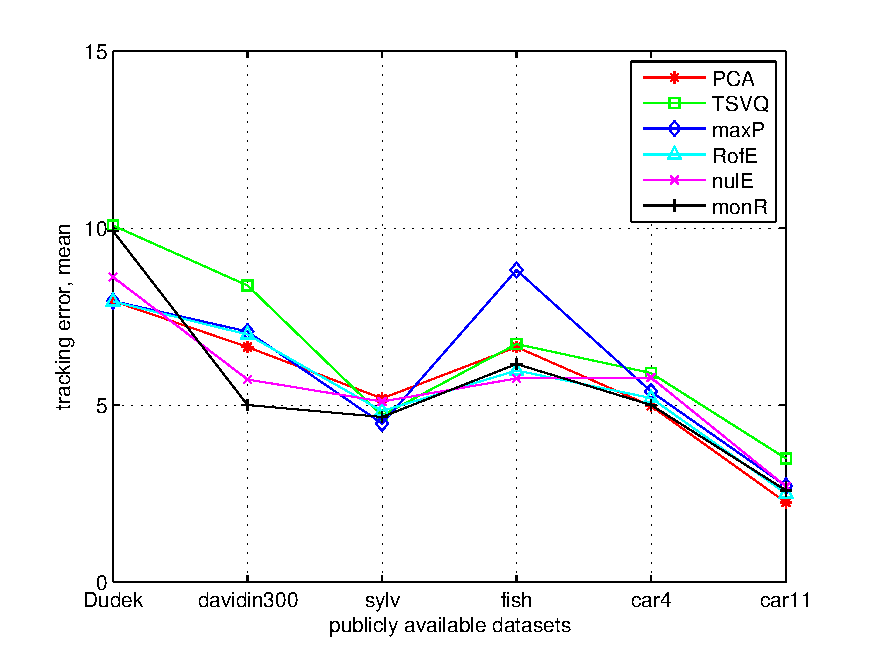
\includegraphics[width=0.47\textwidth]{thesis/results_final_2a_mean.pdf}\label{fig:results_final_2a_mean}}
								\subfigure[\%age of datasets over which best mean tracking error is achieved over all parameters.]{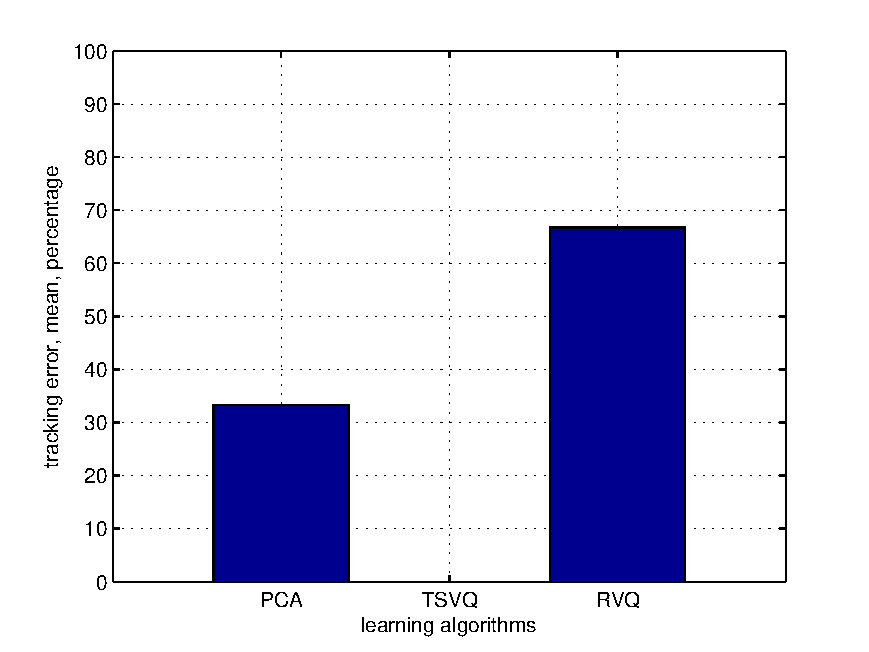
\includegraphics[width=0.47\textwidth]{thesis/results_final_2b_mean_percent.pdf}\label{fig:results_final_2b_mean_percent}}
								\caption{Tracking results (2 of 5), comparison of mean tracking performance.  RVQ performs better over twice as many datasets as PCA.}
								\label{fig:results_final_2_mean}
								\end{figure}


%\begin{enumerate}
%\item \underline{Continually increasing error}.  For Dudek and sylv, the error continues to increase from $Q=8$ to $Q=32$.
%\item \underline{Sharply decreasing, then sharply increasing error}. For davidin300 and fish, the error decreases from $Q=8$ to $Q=16$, and then increases from $Q=16$ to $Q=32$.   The tracking error at $Q=16$ is significantly lower than for $Q=8$ and $Q=32$.
%\item \underline{Mildly decreasing, then mildly increasing error}.  For car4 and car11, like for davidin300 and fish above, the error decreases from $Q=8$ to $Q=16$, and then increases from $Q=16$ to $Q=32$.  However, the drop and rise in error is not as steep.
%\item \underline{Highest error}.  The average error for the Dudek sequence is highest.  This is because this sequence contains more variation than all other sequences including temporary occlusions, expression changes, structured noise, lighting changes and pose changes.  
%\item \underline{Face tracking}.  
%\end{enumerate}

For the Dudek and davidin300 sequences which consist of tracking a face, we look at some related areas in the context of facial processing using PCA, 

\begin{enumerate}
\item \underline{Face reconstruction}.  It has been shown that 40 eigenfaces can be used to reconstruct a face with 3\% error~\cite{1987_JNL_Faces_Sirovich}.
\item \underline{Face recognition}.  Face recognition performance levels off at about 25 principal components, or 45 principal components if the first 3 principal components are dropped~\cite{1997_JNL_EigenVsFisherFaces_Bel}.  The reason for dropping 3 principal components is that~\cite{1992_THE_GeoPhoto_Shashua} showed that for a fixed viewpoint, images of a Lambertian surface\footnote{A Lambertian surface, or informally a matte surface, is a surface that has constant BRDF (bidirectional reflectance distribution function) $\rho(\theta_o, \phi_o, \theta_i, \phi_i)=\frac{L_o(x, \theta_o, \phi_o)}{L_i(x, \theta_i, \phi_i)\cos\theta_i d\omega}$, where the angles ($\theta_o, \phi_o$) define the outgoing light direction and angles ($\theta_i, \phi_i$) define the incoming light direction.  A surface illuminated by radiance $L_i(x, \theta_i, \phi_i)$ coming in from a differential region of solid angle $d\omega$ at angles $\theta_i, \phi_i$ receives irradiance $L_i(x, \theta_i, \phi_i)\cos\theta_i d\omega$.  Irradiance is measured in $\mathrm{W/m^2}$, while the solid angle $d\omega$ is measured in steridians, sr.  The unit of BRDF is therefore $\mathrm{sr^{-1}}$~\cite{2002_BOOK_CV_Forsyth}.} under varying lighting conditions lie in a 3D linear subspace of the high-dimensional image space.
\item \underline{Accounting for lighting changes in face recognition}.  As mentioned above, the first 3 principal components account for lighting changes in faces.  However, these components are unlikely to only account for lighting variation and removing them may result in loss of important information~\cite{1997_JNL_EigenVsFisherFaces_Bel}.
\end{enumerate}

								\begin{figure}[t]
								\centering
								\begin{tabular}{|l|c|c|c|c|c|c|}
\hline
&\textbf{PCA}&\textbf{TSVQ}&\textbf{maxP}&\textbf{RofE}&\textbf{nulE}&\textbf{monR}\\\hline
\textbf{Dudek}&7.81&8.62&7.78&7.11&9.65&11.81\\\hline
\textbf{davidin300}&4.60&12.88&6.84&9.02&7.17&50.00\\\hline
\textbf{sylv}&5.47&4.70&4.00&4.12&4.81&4.31\\\hline
\textbf{fish}&2.17&10.07&11.50&2.96&4.03&2.89\\\hline
\textbf{car4}&4.60&5.11&4.67&4.93&5.28&5.07\\\hline
\textbf{car11}&2.13&2.21&2.17&2.47&2.59&2.47\\\hline
\textbf{ \% best}&66.67&0.00&16.67&16.67&0.00&0.00\\\hline
\end{tabular}

								\subfigure[Tracking error for each algorithm with 16 eigenvectors/code-vectors stored in memory.]{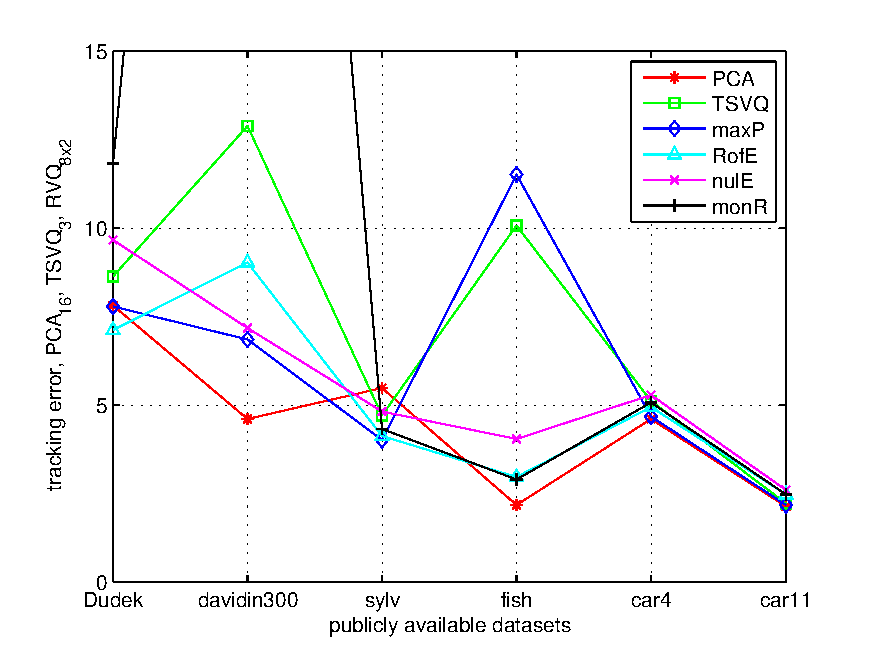
\includegraphics[width=0.47\textwidth]{thesis/results_final_3a_16.pdf}\label{fig:results_final_3a_16}}
								\subfigure[\%age of datasets over which best tracking error is achieved with 16 eigenvectors/code-vectors stored in memory.]{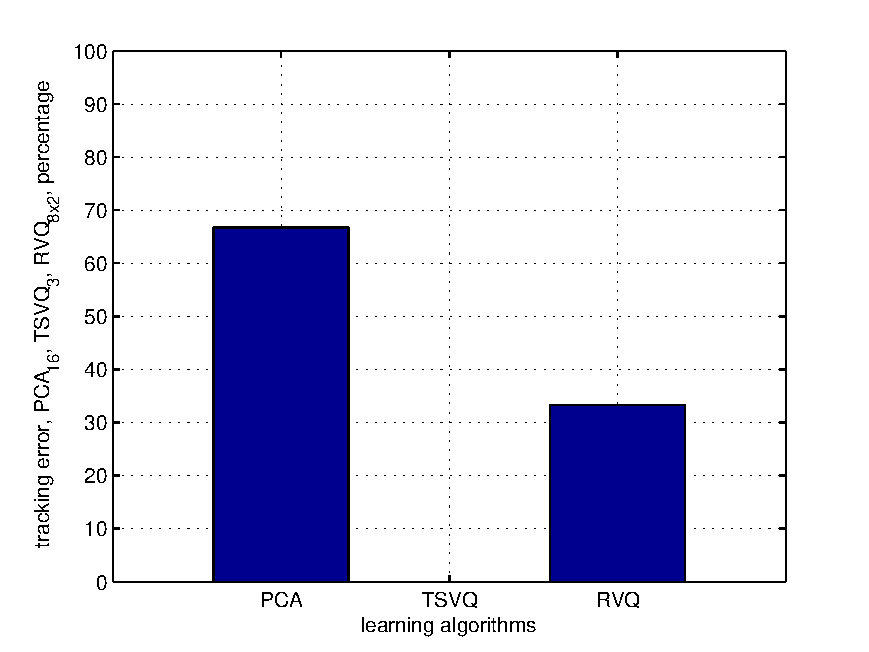
\includegraphics[width=0.47\textwidth]{thesis/results_final_3b_16_percent.pdf}\label{fig:results_final_3b_16_percent}}
								\caption{Tracking results (3 of 5), comparison of tracking performance if 16 eigenvectors/code-vectors are stored in memory.  PCA performs better over twice as many datasets as RVQ.}
								\label{fig:results_final_3_16}
								\end{figure}

Given these observations in related areas of facial processing, we do not remove any principal components.  However, unlike the face recognition case, our tracking performance does not keep increasing till 20 or more eigenvectors.  An important difference in tracking applications however is that face alignment is noisy.  It appears that in the Dudek and davidin300 sequences which have large pose changes, the first few eigenvectors are able to capture the linear dependencies in the slightly shifted faces.  After that, the later eigenvectors explain the residual noise.  This can lead to decreased tracking performance since reconstructions using an eigenspace that partially explains noise will be noisy.  Noisy reconstructions will get inaccurate DFFS (distance-from-feature-space) scores, which in turn will cause incorrect weighting for particle filter candidates in the tracking process.  This will lead to larger tracking error.

								\begin{figure}[t]
								\centering
								\begin{tabular}{|l|c|c|c|c|c|c|}
\hline
&\textbf{PCA}&\textbf{TSVQ}&\textbf{maxP}&\textbf{RofE}&\textbf{nulE}&\textbf{monR}\\\hline
\textbf{Dudek}&8.54&11.87&7.92&8.43&8.19&9.17\\\hline
\textbf{davidin300}&6.93&6.29&4.47&6.21&5.35&5.83\\\hline
\textbf{sylv}&5.72&4.80&4.68&5.54&5.74&4.58\\\hline
\textbf{fish}&7.98&4.59&2.78&12.22&2.48&3.62\\\hline
\textbf{car4}&5.52&6.79&6.38&5.14&5.84&5.18\\\hline
\textbf{car11}&2.39&5.28&2.36&2.33&2.52&2.72\\\hline
\textbf{ \% best}&0.00&0.00&33.33&33.33&16.67&16.67\\\hline
\end{tabular}

								\subfigure[Tracking error for each algorithm with 32 eigenvectors/code-vectors stored in memory.]{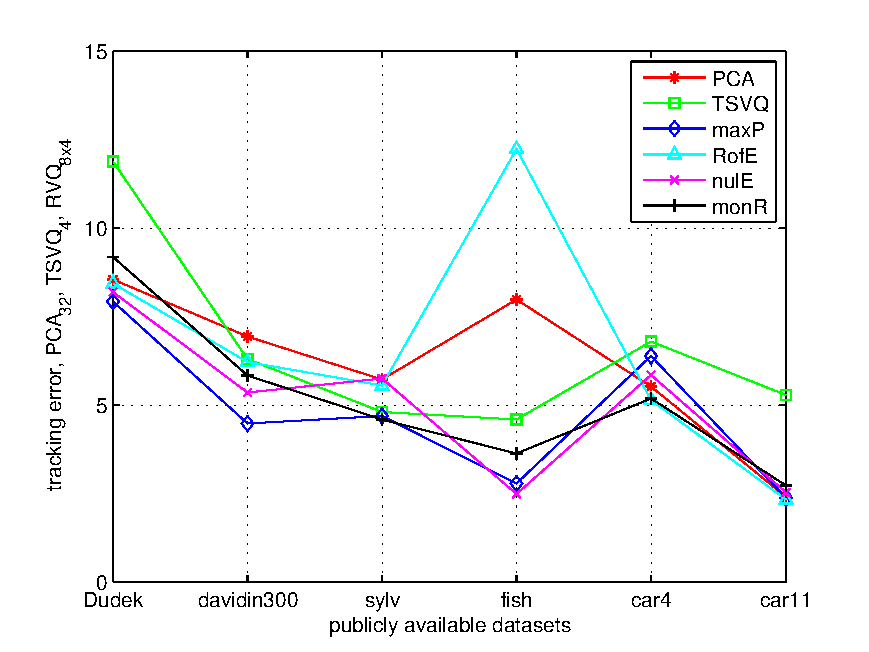
\includegraphics[width=0.47\textwidth]{thesis/results_final_4a_32.pdf}\label{fig:results_final_4a_32}}
								\subfigure[\%age of datasets over which best tracking error is achieved with 32 eigenvectors/code-vectors stored in memory.]{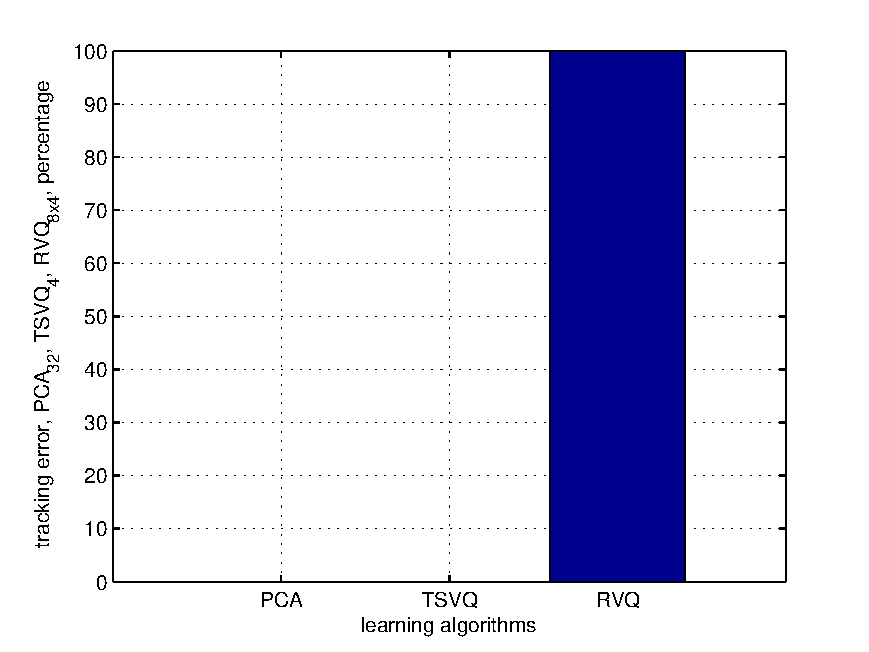
\includegraphics[width=0.47\textwidth]{thesis/results_final_4b_32_percent.pdf}\label{fig:results_final_4b_32_percent}}
								\caption{Tracking results (4 of 5), comparison of tracking performance if 32 eigenvectors/code-vectors are stored in memory.  RVQ performs the best over all datasets.}
								\label{fig:results_final_4_32}
								\end{figure}

%=========================
\section{Results}
%=========================
Our final tracking results are plotted in 5 figures, Figures~\ref{fig:results_final_1_best}, \ref{fig:results_final_2_mean}, \ref{fig:results_final_3_16}, \ref{fig:results_final_4_32} and~\ref{fig:results_final_5_configs}.  These plots are based entirely on detailed plots in Figures~\ref{fig:results_final_pca_}, \ref{fig:results_final_tsvq}, \ref{fig:results_final_maxP}, \ref{fig:results_final_RofE} \ref{fig:results_final_nulE} and \ref{fig:results_final_monR} in Appendix~\ref{App:tracking_error_plots} for PCA, TSVQ, maxP, RofE, nulE and monR respectively.

We start with Figure~\ref{fig:results_final_1_best}.  In this figure, we plot best possible tracking performance for each algorithm.  For PCA, this means the best possible performance attained for each of the datasets for $Q$=8, 16 and 32.  For TSVQ, best possible performance for each dataset is over $P$=3, 4 and 5.  For maxP, RofE, nulE and monR, best possible performance for each dataset is over 8x2, 8x4 and 8x8.  The reason for plotting performance for each dataset separately is that each dataset represents a different distribution and we would like to gauge performance for each algorithm over the different distributions.  We see that performance for PCA and all 4 RVQ based algorithms is very close while TSVQ tracking error is highest in most cases.  

PCA performs best in the fish, car4 and car11 sequences while RVQ performs best in the remaining three datasets, Dudek, davidin300 and sylv.  TSVQ does not perform best in any sequence.  Note that the performance difference between PCA and RVQ in the car4 and car11 sequences is negligible.  Recall that car4 and car11 are relatively benign datasets with little variation in pose and lighting.  The fish sequence has sudden motion as well as sudden global lighting changes.   Since global lighting change induces linear correlation in the data, it makes sense that PCA does well in this sequence.  The reason is that global illumination moves the illuminated object within the modeled PCA subspace~\cite{1987_JNL_Faces_Sirovich}.  For a VQ based method such as RVQ or TSVQ, several codevectors would have to be dedicated to different lighting conditions to model all possible lighting changes.  

RVQ performs best over the Dudek, davidin300 and sylv sequences.  All 3 of these sequences have moderate lighting changes while Dudek and davidin300 have several forms of noise as discussed earlier.  For Dudek, RofE does best.  The reason is that in the presence of uncertainties, RofE holds tight to what has already been modeled and is resistant to accepting sudden changes in the underlying distribution.  It is therefore better able to handle blur and other forms of noise that did not exist in the training data.  On the other extreme is monR which greedily attempts to minimize reconstruction error.  Out of all RVQ methods, this method performs worse, but even then, not by much.  Second best performance is for maxP which is again not a greedy method.  Third best performance is for nulE which is also a greedy method but less so than monR.

								\begin{figure}[h!]
								\centering
	
								\subtable[PCA.]{\begin{tabular}{|c|c|c|c|}
\hline
\textbf{8}&\textbf{16}&\textbf{32}&\textbf{mean}\\\hline
6.15&4.46&6.18&5.60\\\hline
\end{tabular}
}
								\subtable[TSVQ.]{\begin{tabular}{|c|c|c|c|}
\hline
\textbf{3}&\textbf{4}&\textbf{5}&\textbf{mean}\\\hline
7.26&6.60&5.74&6.54\\\hline
\end{tabular}
}
								\subtable[maxP.]{\begin{tabular}{|c|c|c|c|}
\hline
\textbf{8x2}&\textbf{8x4}&\textbf{8x8}&\textbf{mean}\\\hline
6.16&4.76&7.25&6.06\\\hline
\end{tabular}
}
								\subtable[RofE.]{\begin{tabular}{|c|c|c|c|}
\hline
\textbf{8x2}&\textbf{8x4}&\textbf{8x8}&\textbf{mean}\\\hline
5.10&6.64&4.94&5.56\\\hline
\end{tabular}
}
								\subtable[nulE.]{\begin{tabular}{|c|c|c|c|}
\hline
\textbf{8x2}&\textbf{8x4}&\textbf{8x8}&\textbf{mean}\\\hline
5.59&5.02&6.20&5.60\\\hline
\end{tabular}
}
								\subtable[monR.]{\begin{tabular}{|c|c|c|c|}
\hline
\textbf{8x2}&\textbf{8x4}&\textbf{8x8}&\textbf{mean}\\\hline
5.31&5.18&6.19&5.56\\\hline
\end{tabular}
}
								\subtable[maxP, RofE, nulE, monR.]{\begin{tabular}{|c|c|c|}
\hline
\textbf{8x2}&\textbf{8x4}&\textbf{8x8}\\\hline
5.54&5.40&6.15\\\hline
\end{tabular}
}\\
								\subfigure[PCA]{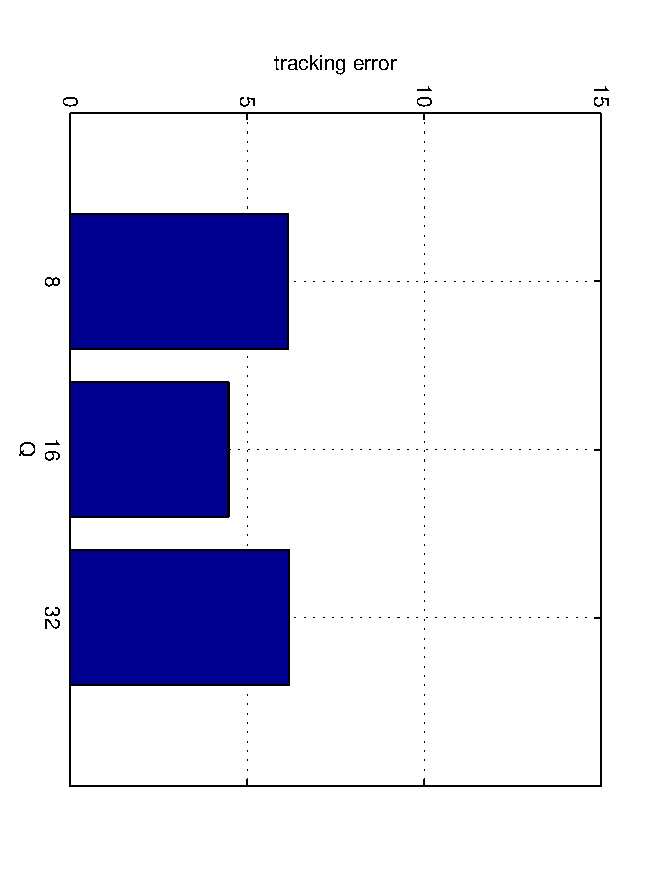
\includegraphics[width=0.225\textwidth, angle=90]{thesis/results_final_5a_pca_.pdf}\label{fig:results_final_5a_pca_}}
								\subfigure[TSVQ.]{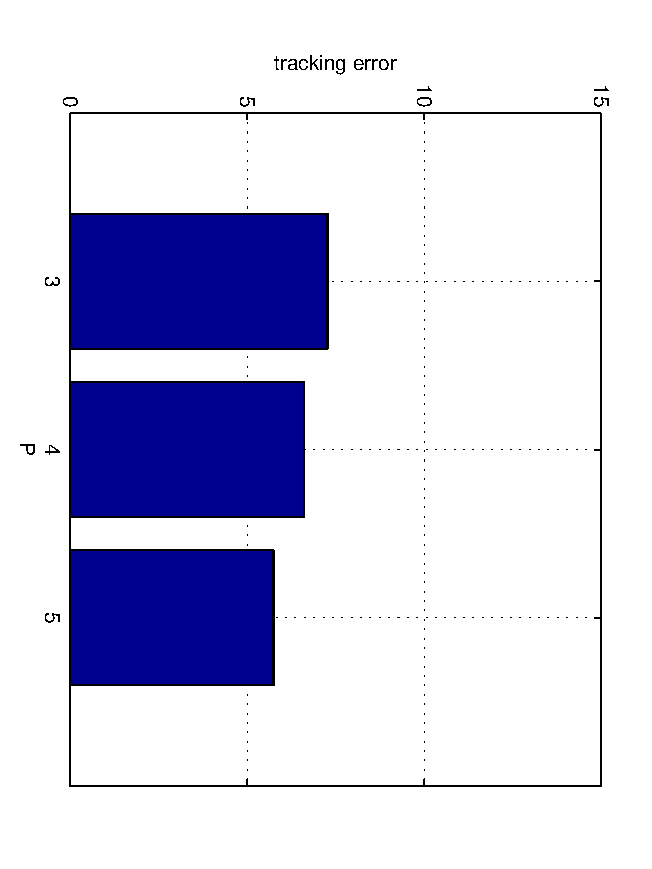
\includegraphics[width=0.225\textwidth, angle=90]{thesis/results_final_5b_tsvq.pdf}\label{fig:results_final_5b}}
								\subfigure[maxP.]{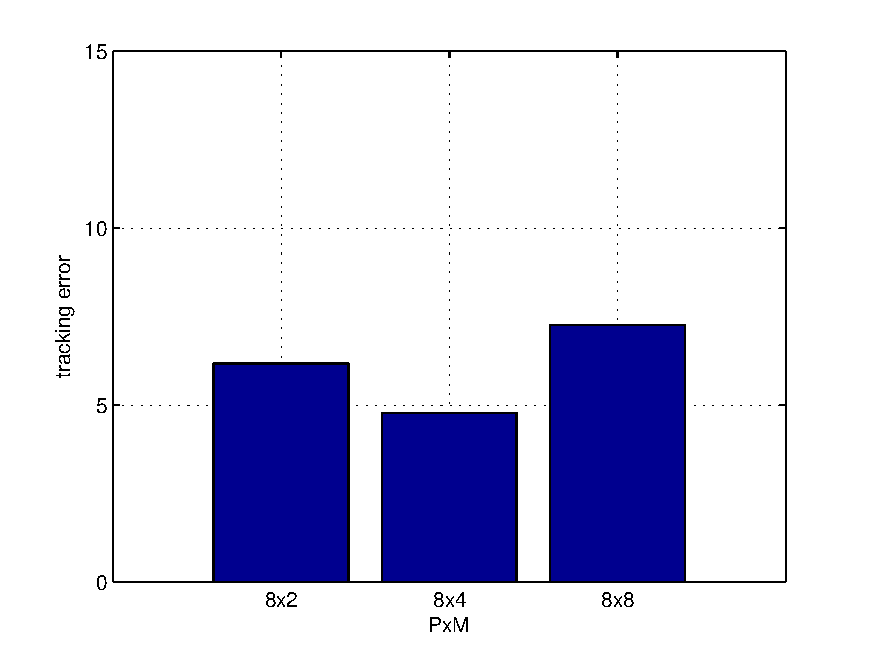
\includegraphics[width=0.3\textwidth]{thesis/results_final_5c_maxP.pdf}\label{fig:results_final_5c}}
								\subfigure[RofE.]{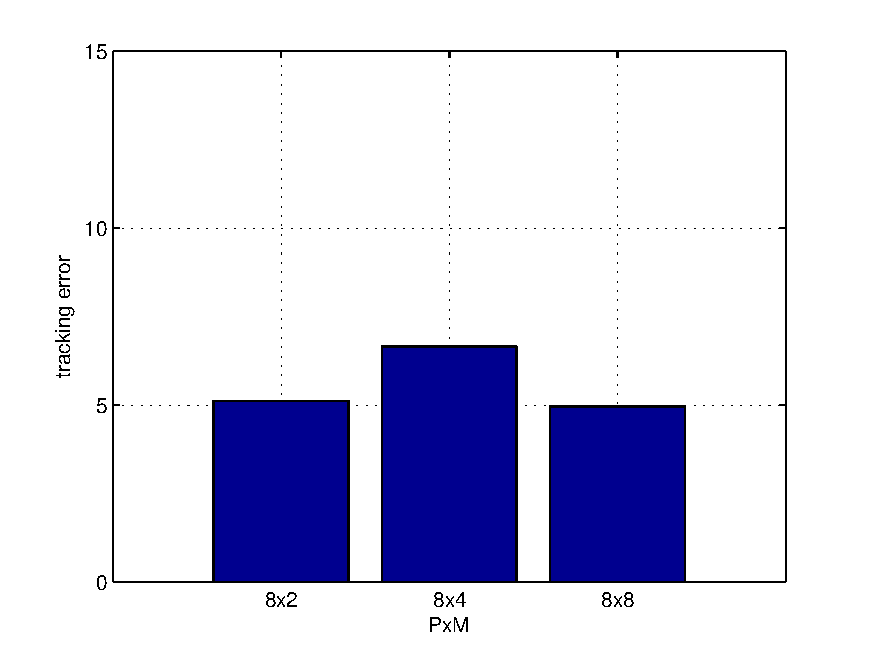
\includegraphics[width=0.3\textwidth]{thesis/results_final_5d_RofE.pdf}\label{fig:results_final_5d}}
								\subfigure[nulE.]{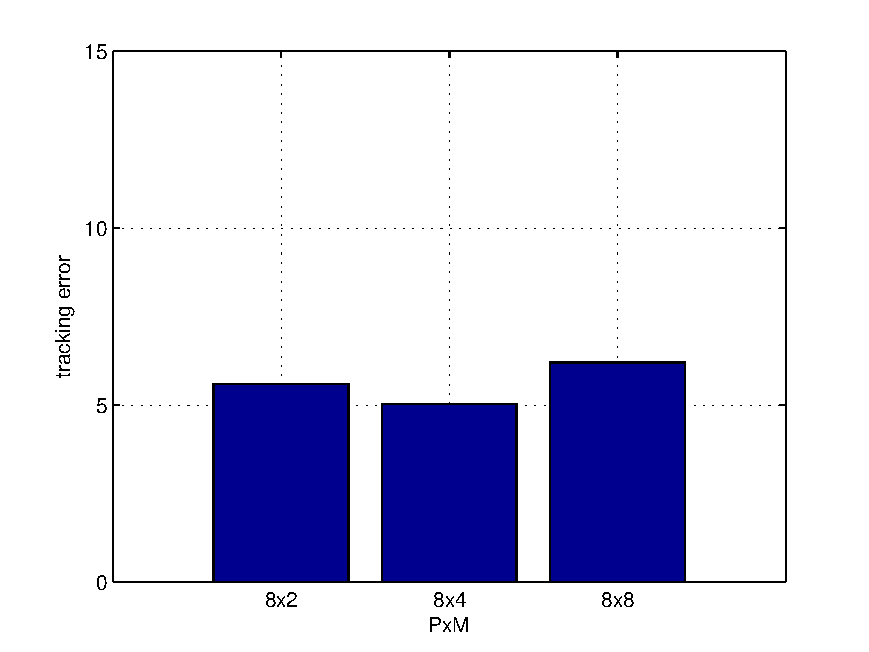
\includegraphics[width=0.3\textwidth]{thesis/results_final_5e_nulE.pdf}\label{fig:results_final_5e}}
							\subfigure[monR.]{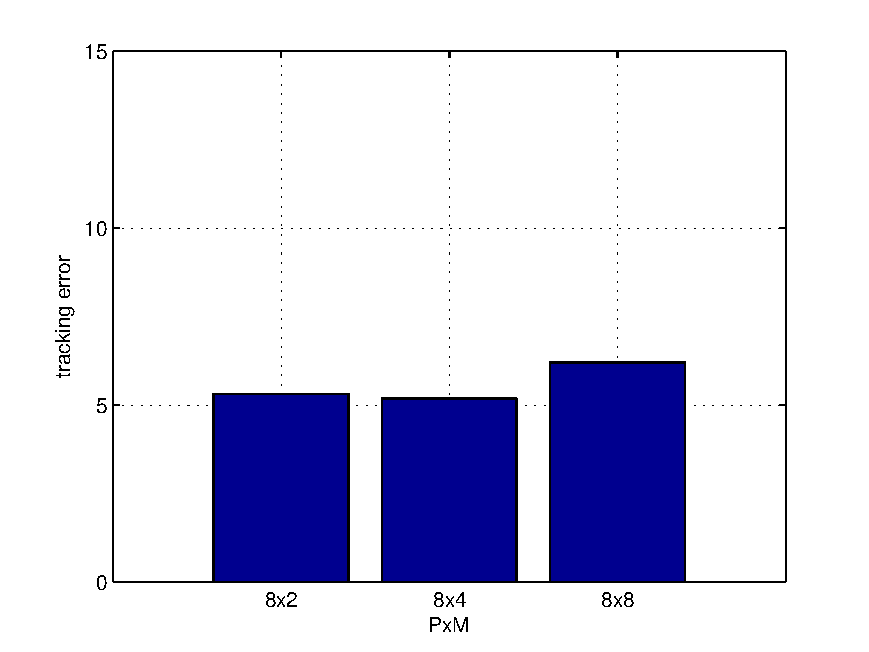
\includegraphics[width=0.3\textwidth]{thesis/results_final_5f_monR.pdf}\label{fig:results_final_5f}}
								\subfigure[maxP, RofE, nulE, monR.]{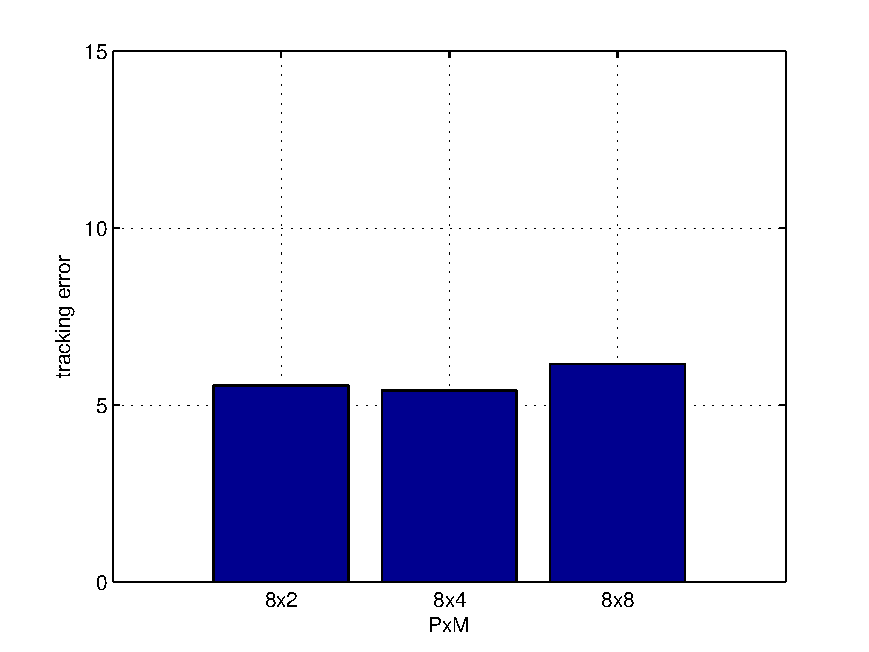
\includegraphics[width=0.3\textwidth]{thesis/results_final_5g_8x2_8x4_8x8.pdf}\label{fig:results_final_5g_8x2_8x4_8x8}}
								\caption{Tracking results (5 of 5), comparison of tracking performance as parameters for each algorithm are varied.  In (d), we see that over all RVQ algorithms, RofE has best mean performance.  In (g) it is clear that the best RVQ configuration is 8x4.}
								\label{fig:results_final_5_configs}
								\end{figure}


We now turn to Figure~\ref{fig:results_final_2_mean}.  In this figure, mean performance over all configurations is shown.  It may be noted that monR loses track in one instance.  That instance is not factored into the means since it is not clear how penalize a lost track when performing mean computations.  Here, we see that RVQ performs best 66.7\% of the time.  This time, in addition to Dudek, davindin300 and sylv, RVQ performs better than PCA in the fish sequence as well.  The reason for this is that PCA is unable to track the fish sequence well when it has too few, i.e., 8 eigenvectors or when it has too many, i.e., 32 eigenvectors.  In the 8 eigenvector case, the subspace does not have enough dimensions to model lighting changes well.  Even though it has been shown, as mentioned earlier, that only 3 eigenvectors are needed to model lighting changes~\cite{1987_JNL_Faces_Sirovich}, in practice this does not hold due to shadowing and specularities~\cite{1997_JNL_EigenVsFisherFaces_Bel}.  For too many eigenvectors, over-fitting is an issue as mentioned in an earlier report.  For $Q=16$, PCA performs best and that is why it had best possible performance.  However, when it comes to means, all 4 RVQ configurations are able to outperform PCA in mean performance.

In Figures~\ref{fig:results_final_3_16} and~\ref{fig:results_final_4_32}, we hold the number of eigenvectors for PCA or codevectors for TSVQ and RVQ constant at 16 and 32 respectively\footnote{This is 15 and 31 actually for TSVQ but we ignore this slight difference.}.  In these figures, we see that PCA outperforms RVQ for 16 vectors but RVQ completely outperforms PCA for 32 vectors.  For a given memory cost, and therefore for a given rate, RVQ overall outperforms PCA.  

Finally, in Figure~\ref{fig:results_final_5_configs}, we plot tracking performance for each algoritm separately for its different configurations.  For 3 configurations per algorithm, $Q$=8, 16, 32 for PCA, $P$=3, 4, 5 for TSVQ and $PxM$ = 8x2, 8x4, 8x8 for RVQ, there are 4 possible outcomes listed below.  Of these, the first 3 are to be expected.  The fourth however requires further scrutiny.

\begin{enumerate}
\item \underline{Monotonically increasing error.}  This would mean that the degrees of freedom (DoF) in the learning algorithm, such as PCA, TSVQ or RVQ, model the underlying distribution well with low DoFs and adding DoFs is leading to over-generalization.  We do not see this performance in any case since we start with low DoFs.  We got an initial estimate of how many DoFs to use using our experiments on appearance modeling that have mentioned in a previous report.
\item \underline{Monotonically decreasing error.}  This happens for TSVQ.  This means that adding more stages to TSVQ may increase performance.  In our case, we use 3, 4 and 5 stages to keep the DoFs in TSVQ close to the DoFs for RVQ and PCA.
\item \underline{Decreasing error followed by increasing error.}  We see this performance for PCA, maxP, nulE and monR.  This is a sign that the correct number of DoFs were chosen and that when error is minimum, the algorithm now has enough capacity to model the underlying distribution, but without over-fitting.
\item \underline{Increasing error followed by decreasing error.}  We see this in one case, RofE, and in some cases in TSVQ in Figure~\ref{fig:results_final_tsvq}.  To see this, consider the example of $K$=2, 4 and 8 code-vectors in $\mathbb{R}$ uniformly spaced on the inteval [0,7].  For $K$=2, the code-vectors are 2.33 and 4.66.  For the $K$=4 case, the code-vectors are 1.4, 2.8, 4.2 and 5.6.  For the $K$=8 case, the code-vectors are $\{0, 1, 2, 3, \ldots, 7\}$.  In regions around 2.33 and 4.6, there are certain contiguous regions where the reconstruction error is greatest for $K$=4.  This shows that although in general, one would not expect reconstruction error, and therefore tracking error to be lowest for an intermediate number of code-vectors $K$, it is possible for a test vector to score highest error for an intermediate $K$.  If this occurs at a point in the tracking process where the target is moving quickly for instance, then a wrong decision can cause tracking error to increase.  In certain cases, it may not be possible to recover from this wrong decision.  See Figures~\ref{fig:results_TSVQ_Dudek_errors}, \ref{fig:results_TSVQ_Dudek_FN10} and \ref{fig:results_TSVQ_Dudek_FN457} in Appendix~\ref{App:TSVQ_Dudek_example} for an example of such a scenario for TSVQ tracking.


\end{enumerate}

%
%For PCA, on average, $Q=16$ produces the lowest tracking error.  On average, the tracking error decreases from $Q=8$ to $Q=16$, and then increases from $Q=16$ to $Q=32$.  It appears that the number of eigenvectors required to capture the linear correlation in these datasets is between 16 and 32, but closer to 16.   







%\begin{table}[h!]
%\centering
%\begin{tabular}{|l|c|c|c|}
\hline
&\textbf{PCA}&\textbf{TSVQ}&\textbf{RVQ}\\\hline
\textbf{Dudek}&7.44&8.62&6.68\\\hline
\textbf{davidin300}&4.60&5.93&4.29\\\hline
\textbf{sylv}&4.34&4.61&4.19\\\hline
\textbf{fish}&2.17&4.59&2.60\\\hline
\textbf{car4}&4.60&5.11&4.72\\\hline
\textbf{car11}&2.13&2.21&2.00\\\hline
\textbf{mean}&4.21&5.18&4.08\\\hline
\end{tabular}

%\caption{Comparison of best possible tracking error between PCA, RVQ and TSVQ over all algorithm parameters for 6 publicly available challenging datasets, Dudek, davidin300, sylv, fish, car4 and car11.  The table shows that RVQ produces the best results for 4 of the 6 datasets.  Overall tracking error is least for RVQ followed by PCA, and then followed by TSVQ.}
%\end{table}
%
%\begin{table}[h!]
%\centering
%\input{thesis/tables_comparison_DOF_16}
%\caption{Comparison of tracking results using the same DoF, 16 eigenvectors for PCA, 8x2 RVQ and 3x2 TSVQ (15 DOF for TSVQ, 8 terminal code-vectors and 7 stage code-vectors).  RVQ has best overall tracking performance.}
%\end{table}
%
%\begin{table}[h!]
%\centering
%\input{thesis/tables_comparison_DOF_32.tex}
%\caption{Comparison of tracking results using the same DoF, 32 eigenvectors for PCA, 8x4 RVQ and 4x2 TSVQ (31 DOF for TSVQ, 16 terminal code-vectors and 15 stage code-vectors).  RVQ has best tracking performance every time, and therefore also best overall performance.}
%\end{table}


For the interested reader, the appendix contains detailed results for tracking errors for all 6 datasets, for all RVQ types (maxQ, RofE, nulE, monR), over several RVQ configurations (8x2, 8x4, 8x8, 8x12, 8x16).  Also, detailed graphical results for all 6 datasets, for all RVQ types, for the 8x4 configuration are also presented.











